\documentclass[multi, tikz, a4paper, oneside]{article}
\usepackage[utf8]{inputenc}
\usepackage{makecell}
\usepackage{tikz}
\usepackage{graphicx}
\usepackage{grffile}
\usepackage{amssymb}% http://ctan.org/pkg/amssymb
\usepackage{pifont}% http://ctan.org/pkg/pifont
\newcommand{\cmark}{\ding{51}\space}%
\newcommand{\xmark}{\ding{55}\space}%
\usepackage{hyperref}

\usepackage[demo]{graphicx}
\usepackage{subcaption}

\usepackage{etoc}


%%%%%%%%%%%%%%%%%%%%% SVG %%%%%%%%%%%%%%%%%%%%%%%
\usepackage{ifluatex}
\ifluatex
\usepackage{pdftexcmds}
\makeatletter
\let\pdfstrcmp\pdf@strcmp
\let\pdffilemoddate\pdf@filemoddate
\makeatother
\fi
\usepackage{svg}

%%%%%%%%%%%%%%%%%%%%% Bibliography %%%%%%%%%%%%%%%%%%%%%%%%
\usepackage{biblatex}
\addbibresource{references.bib}

%%%%%%%%%%%%%%%%%%%%% HTML %%%%%%%%%%%%%%%%%%%%%%%%%
\usepackage{color}
\definecolor{editorGray}{rgb}{0.95, 0.95, 0.95}
\definecolor{editorOcher}{rgb}{1, 0.5, 0} % #FF7F00 -> rgb(239, 169, 0)
\definecolor{editorGreen}{rgb}{0, 0.5, 0} % #007C00 -> rgb(0, 124, 0)
\usepackage{upquote}
\usepackage{listings}

\usepackage{listings}
\usepackage{color}
\definecolor{lightgray}{rgb}{.9,.9,.9}
\definecolor{darkgray}{rgb}{.4,.4,.4}
\definecolor{purple}{rgb}{0.65, 0.12, 0.82}
\definecolor{brightpink}{rgb}{1.0, 0.0, 0.5}
\definecolor{orange}{rgb}{255,165,0}


\lstdefinelanguage{JavaScript}{
  keywords={const, genSaltSync, hashSync, json, save, then, then, typeof, new, true, false, catch, function, return, null, catch, switch, var, if, in, while, do, else, case, break},
  keywordstyle=\color{blue}\bfseries,
  ndkeywords={class, export, boolean, throw, bcrypt, implements, import, this, User, username, password, email, message, data, body},
  ndkeywordstyle=\color{brightpink}\bfseries,
  identifierstyle=\color{black},
 % keywordstyle = [2]{\color{orange}},
%  morekeywords = [2]{;},
  sensitive=false,
  comment=[l]{//},
  morecomment=[s]{/*}{*/},
  commentstyle=\color{darkgray}\ttfamily,
  stringstyle=\color{red}\ttfamily,
  morestring=[b]',
  morestring=[b]"
}


\lstdefinelanguage{HTML5}{
        language=html,
        sensitive=true,
        alsoletter={<>=-},
        otherkeywords={
        % HTML tags
        <html>, <head>, <title>, </title>, <meta, />, </head>, <body>,
        <canvas, \/canvas>, <script>, </script>, </body>, </html>, <!, html>, <style>, </style>, ><
        },
        ndkeywords={
        % General
        =,
        % HTML attributes
        charset=, id=, width=, height=,
        % CSS properties
        border:, transform:, -moz-transform:, transition-duration:, transition-property:, transition-timing-function:
        },
        morecomment=[s]{<!--}{-->},
        tag=[s]
}

\lstset{%
    % Basic design
    backgroundcolor=\color{editorGray},
    basicstyle={\small\ttfamily},
    frame=l,
    % Line numbers
    xleftmargin={0.75cm},
    numbers=left,
    stepnumber=1,
    firstnumber=1,
    numberfirstline=true,
    % Code design
    keywordstyle=\color{blue}\bfseries,
    commentstyle=\color{darkgray}\ttfamily,
    ndkeywordstyle=\color{editorGreen}\bfseries,
    stringstyle=\color{editorOcher},
    % Code
    language=HTML5,
    alsolanguage=JavaScript,
    alsodigit={.:;},
    tabsize=2,
    showtabs=false,
    showspaces=false,
    showstringspaces=false,
    extendedchars=true,
    breaklines=true,
    % Support for German umlauts
    literate=%
    {Ö}{{\"O}}1
    {Ä}{{\"A}}1
    {Ü}{{\"U}}1
    {ß}{{\ss}}1
    {ü}{{\"u}}1
    {ä}{{\"a}}1
    {ö}{{\"o}}1
}

\usepackage{listings}

% Define a custom style for HTML code
\lstdefinestyle{htmlstyle}{
  language=HTML,
  basicstyle=\small\ttfamily,
  tabsize=4,
  frame=single,
  breaklines=true,
  keywordstyle=\color{blue},
  commentstyle=\color{green!40!black},
  stringstyle=\color{red},
  morekeywords={html, head, title, body, p, a, div}
}

%%%%%%%%%%%%%%%%%%%%%% UEQ %%%%%%%%%%%%%%%%%%%%%%%%%%
\usepackage{pgfplots}
\usepackage{filecontents}



%%%%%%%%%%%%%%%%%%%%%%% YAML %%%%%%%%%%%%%%%%%%%%%%%%%%%
\usepackage{xcolor}
\usepackage{listings}

\usepackage{listingsutf8}

\lstdefinelanguage{docker}{
  keywords={FROM, RUN, COPY, ADD, ENTRYPOINT, CMD,  ENV, ARG, WORKDIR, EXPOSE, LABEL, USER, VOLUME, STOPSIGNAL, ONBUILD, MAINTAINER},
  keywordstyle=\color{blue}\bfseries,
  identifierstyle=\color{black},
  sensitive=false,
  comment=[l]{\#},
  commentstyle=\color{purple}\ttfamily,
  stringstyle=\color{red}\ttfamily,
  morestring=[b]',
  morestring=[b]"
}

\lstdefinelanguage{docker-compose}{
  keywords={image, environment, ports, container_name, ports, volumes, links},
  keywordstyle=\color{blue}\bfseries,
  identifierstyle=\color{black},
  sensitive=false,
  comment=[l]{\#},
  commentstyle=\color{purple}\ttfamily,
  stringstyle=\color{red}\ttfamily,
  morestring=[b]',
  morestring=[b]"
}
\lstdefinelanguage{docker-compose-2}{
  keywords={version, volumes, services},
  keywordstyle=\color{blue}\bfseries,
  keywords=[2]{image, context, environment, ports, container_name, hostname, working_dir, ports, links, build},
  keywordstyle=[2]\color{olive}\bfseries,
  identifierstyle=\color{black},
  sensitive=false,
  comment=[l]{\#},
  commentstyle=\color{purple}\ttfamily,
  stringstyle=\color{red}\ttfamily,
  morestring=[b]',
  morestring=[b]"
}

\lstset{basicstyle=\ttfamily,
  showstringspaces=false,
  commentstyle=\color{red},
  keywordstyle=\color{blue},
  inputencoding=utf8,
  extendedchars=true
}

\lstdefinestyle{yaml}{
  basicstyle=\color{blue}\footnotesize,
  rulecolor=\color{black},
  string=[s]{'}{'},
  stringstyle=\color{blue},
  comment=[l]{:},
  commentstyle=\color{black},
  morecomment=[l]{-}
}


%%%%%%%%%%%%%%%%%%%%%%%% FOREST %%%%%%%%%%%%%%%%%%%%%%%%%
\usepackage{tikz}
\usetikzlibrary{trees}
\usepackage[edges]{forest}
\usepackage{sectsty}
\usepackage{array}
\usepackage{multicol}
\usepackage{graphicx}
\definecolor{folderborder}{RGB}{110,144,169}
\definecolor{folderbg}{rgb}{0.91, 0.84, 0.42}
\usepackage[T1]{fontenc}
\usepackage[utf8]{inputenc} 
\usepackage{floatrow}
\newlength\Size
\setlength\Size{4pt}
\tikzset{%
  folder/.pic={%
    \filldraw [draw=folderborder, top color=folderbg!50, bottom color=folderbg] (-1.05*\Size,0.2\Size+5pt) rectangle ++(.75*\Size,-0.2\Size-5pt);
    \filldraw [draw=folderborder, top color=folderbg!50, bottom color=folderbg] (-1.15*\Size,-\Size) rectangle (1.15*\Size,\Size);
  },
  file/.pic={%
    \filldraw [draw=folderborder, top color=folderborder!5, bottom color=folderborder!10] (-\Size,.4*\Size+5pt) coordinate (a) |- (\Size,-1.2*\Size) coordinate (b) -- ++(0,1.6*\Size) coordinate (c) -- ++(-5pt,5pt) coordinate (d) -- cycle (d) |- (c) ;
  },
}
\forestset{%
  declare autowrapped toks={pic me}{},
  pic dir tree/.style={%
    for tree={%
      folder,
      font=\ttfamily,
      grow'=0,
    },
    before typesetting nodes={%
      for tree={%
        edge label+/.option={pic me},
      },
    },
  },
  pic me set/.code n args=2{%
    \forestset{%
      #1/.style={%
        inner xsep=2\Size,
        pic me={pic {#2}},
      }
    }
  },
  pic me set={directory}{folder},
  pic me set={file}{file},
}
%\newcommand\fname[2]{#1}
\newcommand{\fname}[2]{\begin{tabular}{m{1cm}@{\quad}m{4cm}}#1 & {\color{red}\normalfont#2}\end{tabular}}

\forestset{
  arrow to next tree/.code={
    \draw[dashed] (current bounding box.south east) -- ++(1.5em,0);
    \draw[->](current bounding box.south east) ++(0.25em,0) -- ++(1.5em,0) -- (current bounding box.north east) -- ++(1.5em,0);
  },
  dots below/.style={
    for group={#1}{
      tempdima/.option=y,
      for next node={
        for ancestors={
          TeX={%
            \draw([xshift=\forestregister{folder indent}].parent anchor)--([xshift=\forestregister{folder indent}]\forestoption{x},\forestregister{tempdima}) node[anchor=north]{\vdots};
          },
        },
      },
    },
  },
  prepare fake ancestors/.style={
    for group={#1}{
      init prepare fake parent,
      prepare fake ancestors',
    },
  }, 
  prepare fake ancestors'/.style={
    if nodewalk valid={parent}{
      for parent={
        prepare fake parent,
        prepare fake ancestors',
      },
    }{},
  },
  init prepare fake parent/.style={
    tempdima/.option=y,
  },
  prepare fake parent/.style={
    y/.register=tempdima, y+=10pt,
    coordinate, edge label={}, no edge,
    tikz={\node at ()[anchor=south,xshift=\forestregister{folder indent}]{\vdots};},
    typeset node,
  },
  draw part of tree/.style 2 args={
    for nodewalk={#1,tempcounta/.option=id}{},
    for nodewalk={#2,tempcountb/.option=id}{},
    draw@part@of@tree/.process=RR{tempcounta}{tempcountb},
  },
  draw@part@of@tree/.style 2 args={
    draw tree processing order/.nodewalk style={
      id=#1,
      ancestors,
      fake={id=#1},
      do until={id()==#2}{next node},
    },
    for root'={
      post draw tree hook/.style={},
      for id={#2}{
        if nodewalk valid={next node}{
          post draw tree hook/.append style={
            to be continued={id=#1}{id=#2},
          },
        }{}
      },
      prepare fake ancestors={id=#1},
      draw tree,
    },
  },
  declare count register=current first node,
  draw linear split tree/.style={
    draw tree method/.append style={post draw tree hook},
    begin draw/.append code={[baseline=(current bounding box.north)]},
    draw tree stage/.style={},
    for root'={current first node/.option=id},
    before typesetting nodes/.process=Ow{id}{
      draw tree stage/.append style={
        draw part of tree={id/.register=current first node}{root',last leaf},
      },
    },
  },
  split here/.style={
    draw tree stage/.append style/.process=ROw2{current first node}{id}{
      draw part of tree={id=##1}{id=##2,previous node},
    },
    current first node/.option=id,
  },
}


%%%%%%%%%%%%%%%%%%%%%%%%%%%%%%%%%%%%%%%%%%%%%%%%%%%%%%%%%%%

\usepackage[a4paper,
  bindingoffset=0.2in,
  left=1in,
  right=1in,
  top=1in,
  bottom=1in,
  footskip=.25in]{geometry}

\title{
    Docker Web Interface \\
    \large Applicazioni e Servizi Web
}

\author{Razvan Florian Vasile - 000725342
  \{razvanflorian.vasile@studio@unibo.it\}} \date{01 October 2023}

\usepackage{natbib}
\usepackage{graphicx}

% \setcounter{secnumdepth}{0} % sections are level 1
\begin{document}

\maketitle
\newpage
\tableofcontents
\newpage
\listoffigures
\newpage
\listoftables
\newpage
%%%%%%%%%%%%%%%%%%%%%%
%% \newpage         %%
%% \tableofcontents %%
%% \begin{appendix} %%
%%   \listoffigures %%
%%   \listoftables  %%
%% \end{appendix}   %%
%% \newpage         %%
%%%%%%%%%%%%%%%%%%%%%%
\section{Introduction}
\subsection{Domain}
\paragraph{What is Docker?}
Docker is a containerization platform that allows to package and distribute
applications and their dependencies in a standardized unit called a "container".

\paragraph{What is a container?}
A container is a standard unit of software that packages up code and all its
dependencies so the application runs quickly and reliably from one computing
environment to another.

\paragraph{Def. Dockerfile.}
A Dockerfile is used to define the image of a single container (that is the
template for creating a container starts off by creating an instance of an
image). It provides a set of instructions for building a Docker image, including
specifying the base image, copying files into the image, installing
dependencies, and configuring the container environment.

\paragraph{Example.} It follows an example of how to create an image starting from a Dockerfile. After
the image has been created, it is possible to create an arbitrary number of
independent containers.
\begin{lstlisting}[language=Docker,caption={Sample Dockerfile},breaklines=true,label={code:compose}]
# base environment for our image
FROM node:7-alpine

# container exposes this port (accessible from the host)
EXPOSE 1337

# copy files from host to the container
ADD hello.js /opt/

# start a service
CMD ["node", "/opt/hello.js"]
\end{lstlisting}

\paragraph{Def. docker-compose file.}
Docker Compose is a tool that helps define and share multi-container
applications. With docker-compose, it is possible to create a YAML file to
define each service and with a single command, to launch all services or tear
them all down.

\paragraph{Example.}
Below is an example of a docker-compose.yml file. Firstly, each
docker-compose.yml file needs either an image obtained from the Docker Hub
repository to instantiate containers or alternatively, a Dockerfile defined
locally which serves the same purpose.

\begin{lstlisting}[language=docker-compose-2,caption={Sample docker-compose file},breaklines=true,label={code:compose}]
version: '3.3'

services:
  # defines an arbitrarily service name
  node:
    build:
      # defines locally where the Dockerfile is located
      context: app
      # alternatively, using a remote image
      image: my-remote-img
    ports:
      # ports expose in the <host>:<container> format
      - "1337:1337"
\end{lstlisting}

\paragraph{Relevance with the project.}
In this application, these files represent the building blocks for managing
containers. Essentially, the application parses the {\em{docker-compose}} files
stored at a predefined location ({\textbf{/server-side/docker-projects}}) and
allows them to perform operations such as launching all services, tear them all
down, getting logs of running containers and so on.


\subsection{Benefits of using a GUI}
Firstly, the purpose of this application is to serve as a graphical user
interface to managing docker containers and services. There exist various
benefits of using a GUI as opposed to using only the CLI.

\begin{itemize}
\item Ease of Use for Beginners: GUIs provide a more visually intuitive way to
  interact with containers, making it easier for beginners.
\item Visual Representation: GUIs typically offer a visual representation of
  containers. This can be helpful for quickly grasping the architecture across
  different components.
\item Monitoring and Management: GUIs include built-in monitoring and management
  tools that provide real-time information about container resource usage and
  logs.
\end{itemize}

\section{Requirements}
\paragraph{Requirements Engineering.}
User stories and design tasks were created during the initial phase of the
project. These proved to be essential to make the transition to wireframes and
prototypes using Figma. Subsequently, these mock-ups were transformed into code.

\subsection{User stories}
\label{sec:stories}
\paragraph{Definition.}
User stories are a fundamental concept in Agile software development. They are
informal descriptions of a software feature or functionality from the
perspective of an end user. User stories are used to capture the "who," "what,"
and "why" of a software requirement in a simple and understandable format.

\paragraph{Purpose.}
They are useful because they offer flexibility and simplicity. On top of this
they are user centric which offers value in terms of being able to prioritize
and then incrementally develop the software. By using them, the software
engineers obtain continuous feedback from stakeholders and end users, which
helps in refining and improving the product over time.

Below is a summary of all the user stories that were created. These have a 1 to
1 correspondence with the requirements that were crafted during the proposal of
the project.
\begin{table}[!ht]
    \centering
    \resizebox{1\textwidth}{!}{%
      \begin{tabular}{|l|l|l|l|l|l|l|}
        \hline
        \textbf{ID} & \textbf{Priority} & \textbf{Type} & \textbf{As a $<$type of user$>$} & \textbf{I want to $<$perform some task$>$} & \textbf{So that I can $<$achieve some goal$>$} \\ \hline
        1 & Low & Home Page & First-time visitor & \makecell{Quickly understand what Docker-UI offers} & \makecell{Decide if the application is relevant to me.} \\ \hline
        2 & Low & Documentation Page & Inexperienced user & \makecell{User-friendly documentation page} & \makecell{Easily learn what features the website offers.} \\ \hline
        3 & Medium & Login/Signup Page & New member & \makecell{Seamlessly load previous sessions' content} & \makecell{Be satisfied and make decisions \\based on previous data.} \\ \hline
        4.1 & High & Dashboard Page & Registered user & \makecell{Centralized dashboard to interact with a \\ container’s actions} & \makecell{Manage created containers during\\ their execution.} \\ \hline
        4.2 & High & Dashboard Functionality & Docker user & \makecell{Customize projects maintained by DockerUI} & \makecell{Manipulate docker containers via \\docker-compose files.} \\ \hline
        5 & High & Logger's Page & Experienced user & \makecell{See logging messages within the browser} & \makecell{Easily debug running containers.} \\ \hline
        6 & Medium & Docker Hub & Product owner & \makecell{Simply distribute Docker UI} & \makecell{Dispense the application quickly to \\interested users.} \\ \hline
      \end{tabular}%
    }%
    \caption{User stories}
\end{table}%

\subsection{Design tasks}
\label{sec:tasks}
\paragraph{Definition.}
Design tasks are specific, actionable items that are part of the software
development process. These tasks are focused on creating the visual and
interactive design elements of the software via Figma.

\paragraph{Purpose.}
Design tasks involved the specific activities of creating wireframes and mockups
via Figma. They defined the user interface (UI) and user experience (UX)
aspects. They ensure that the user stories are translated into tangible design
elements.

\begin{table}[!ht]
    \centering
    \resizebox{1\textwidth}{!}{%
      \begin{tabular}{|l|l|l|}
        \hline
        \textbf{ID} & \textbf{Type} & \textbf{Design Steps} \\ \hline
        1 & Home Page &
        \makecell[l]{
          \cmark 1.1. Display a clear and catchy headline that describes our value proposition.\\
          \cmark 1.2. Include a captivating hero image or illustration that resonates with the brand.\\
          \cmark 1.3. Add a login button that guides users to explore further.
        }\\ \hline
        2 & Documentation Page &
        \makecell[l]{
          \xmark 2.1. Setup and host documentation pages via Github Pages (see 2.2).\\
          \cmark 2.2. Setup README.md on Github with information about the project. TODO\\
          \cmark 2.3. Organize the documentation in an easily understandable format.\\
          \cmark 2.4. Provide information on how the website is organized.\\
        }
        \\ \hline
        3 & Login/Signup Page &
        \makecell[l]{
          \cmark 3.1. Offer a clear login form with fields for id and password.\\
          \cmark 3.2. Offer a clear registration page with fields for id, password and email.\\
          \xmark 3.3. Allow users to sign up using social media accounts for convenience (not initial requirement).\\
          \xmark 3.4. Provide password recovery options and ensure a secure login process (not initial requirement).
        }
             \\ \hline
        4.1 & Dashboard design &
        \makecell[l]{
          \cmark 4.1.1. Design a clean and organized dashboard layout using Figma \footnote{Figma Design Page: \href{https://www.figma.com/file/TGgkRNt5faxYmILkp60JdN/Docker-UI?type=design&node-id=0-1&mode=design&t=rZRXwLEom6yfP9AU-0}{here}}.\\
          \cmark 4.1.2. Display account information and settings through intuitive and easy to use icons and widgets.\\
          \cmark 4.1.3. Ensure easy navigation between different sections or features.\\
        }
          \\ \hline
        4.2 & Dashboard Functionaity &
        \makecell[l]{
          \cmark 4.2.1. buildAll(path) - Used to build all services given a Docker Compose file.\\
          \cmark 4.2.2. logs(services, path) uses configServices(path) - Show logs of service(s).\\
          \cmark 4.2.3. kill(path) - Force stop service containers.\\
          \cmark 4.2.4. stop(path) - Stop running containers without removing them.\\
          \cmark 4.2.5. start or restartAll(path) - Restart all services.\\
          \cmark 4.2.6. upAll(path) - Build, (re)creates, starts, and attaches to containers for all services.\\
          \cmark 4.2.7. down(path) - Stops containers and removes containers, networks, volumes, and images created by up.
        }
        \\ \hline
        5 & Logger's Page &
        \makecell[l]{
          \cmark 5.1. Redirect container logging messages to the browser to easily read them.\\
          \cmark 5.2. Create an intuitive interface that allows users to easily navigate across the available features.\\
          \cmark 5.3. Decide on the technologies necessary to setup the real time interaction between the client and server.
        }
        \\ \hline
        6 & Docker Hub &
        \makecell[l]{
          \cmark 6.1. Gain the technical expertise needed to setup a Docker Hub release through existing examples. \\
          \cmark 6.2. Setup dependent containers that need to be installed along-side Docker-UI.\\
          \cmark 6.3. Exhaustive tests on multiple machines to ensure that the release works consistently across different OSes. TODO
        }
        \\ \hline
    \end{tabular}
    }%
    \caption{Design tasks}
    \label{table:tasks}
\end{table}%

\paragraph{Comparison of the two.}

\textbf{User stories} provide the high-level requirements and goals, guiding
what needs to be achieved. They give the 'what' and 'why'. \textbf{Design
  tasks}, on the other hand, provide the 'how' and 'what it looks like'. They
take the user stories and break them down into design elements that fulfill the
user's needs.

\section{Design}

\subsection{MVC}
\label{sec:mvc-design}
The MVC design pattern was used alongside the MEAN technological stack. Below is a
quick overview of both and how they are organized.

\begin{itemize}
\item Model (MongoDB). The model layer is responsible for the application's data
  logic and storing and retrieving data from back-end data stores. In this
  project the data schema and models were defined using Mongoose (a ODM - Object
  Document Mapper).

\item View (Angular). The view layer provides the UI necessary to interact with
  the application. In this project, it is handled by Angular to create a
  frontend UI. The Angular services are used to interact with the Express.js
  controllers via HTTP requests.

\item Controller (Express.js). The controller layer contains the application
  logic necessary to facilitate communication across the application, acting as
  an interface between the view and model layers. Routes were defined as
  endpoints in the \textbf{/roots/server-side/routes} folder.
\end{itemize}

\begin{figure}[h!]
  \centering
  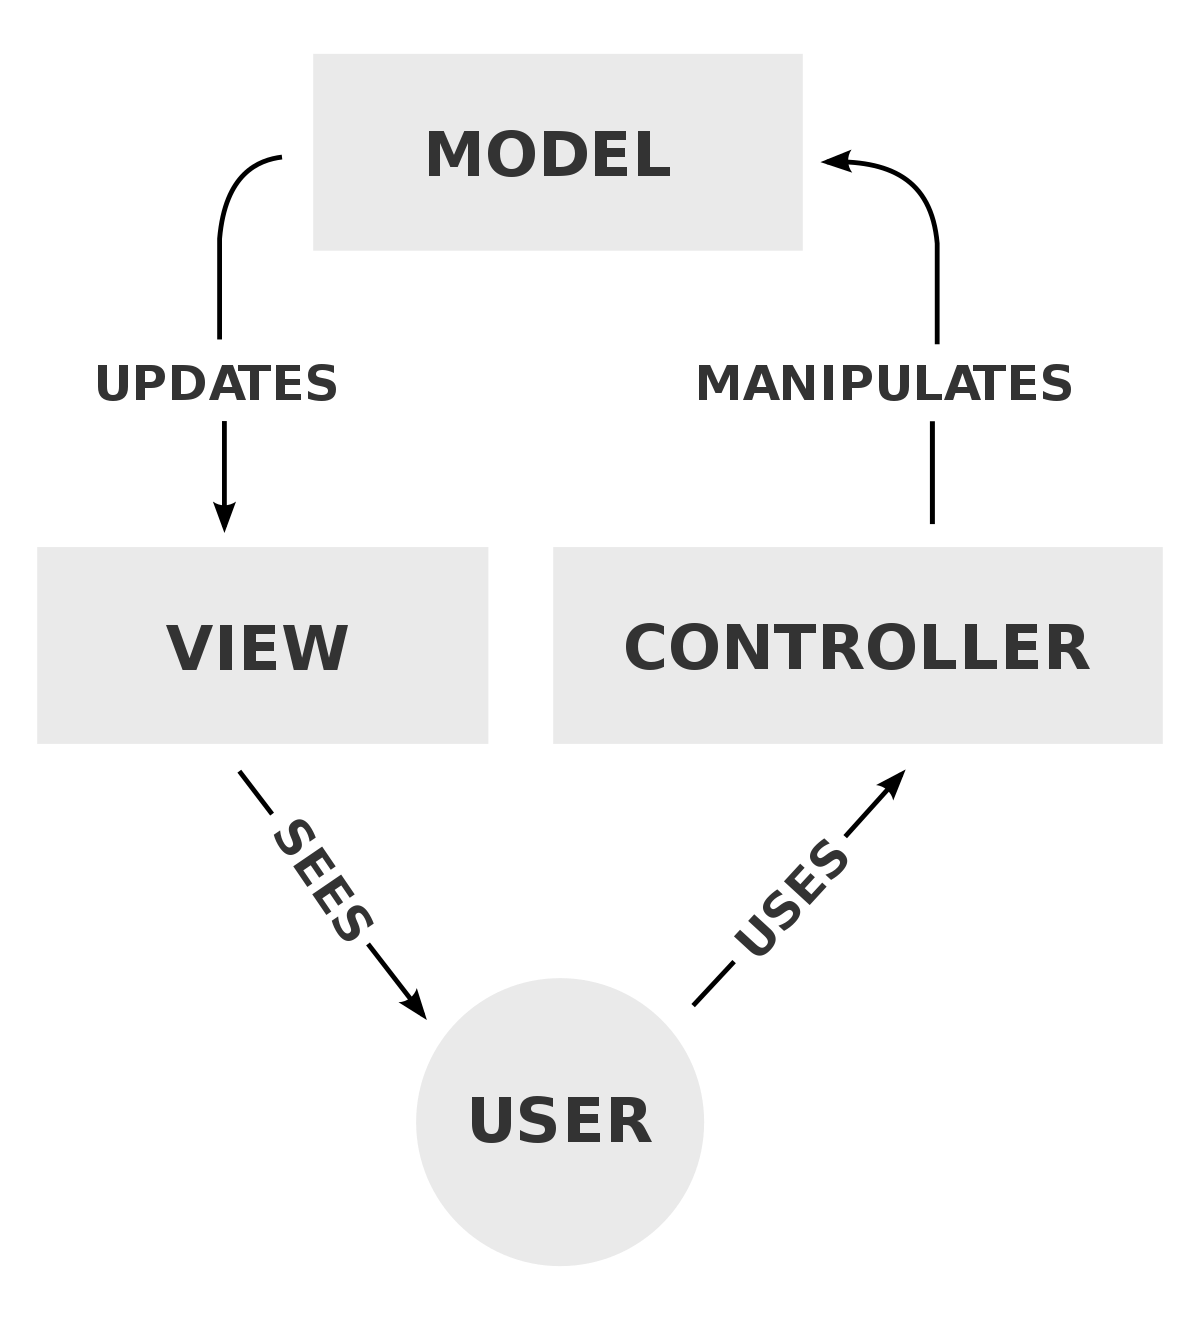
\includegraphics[scale=0.17]{diagrams/MVC}
  \caption{MVC Pattern}
  \label{fig:mvc2}
\end{figure}


\begin{figure}[h]
  \centering
  \begin{forest}
    pic dir tree,
    for descendants={% folder icons by default; override using file for file icons
      directory,
    },
    draw linear split tree,
    to be continued/.style 2 args={
      dots below={#2},
      arrow to next tree,
    },
    [root
      [...]
      [client-side
        [src
          [\fname{app}{View}
            [..., file]
          ]
        ]
      ]
      [server-side
        [\fname{controllers}{\quad\quad\quad Controller}
          [container.controller.js, file]
          [user.controller.js, file]
        ]
        [\fname{docker-projects}{}]
        [\fname{models}{Model}
          [container.model.js, file, split here]
          [project.model.js, file]
          [user.model.js, file]
        ]
        [\fname{routes}{Express.js Routes}
          [container.js, file]
          [user.js, file]
        ]
        [services
          [dockerAdapter.service.js, file]
          [fileSystem.service.js, file]
          [socketIO.service.js, file]
        ]
      ]
    ]
  \end{forest}
  \caption{Code organization under MVC}\label{fig:mvc}
\end{figure}

\label{sec:mvc}
\paragraph{Benefits.}
Some of the benefits of using MVC include organizing the code to enforce a clear
separation of concerns. The view is responsible for presenting the data to the
user, the model represents the application's data and business logic and the
controller handles user input and manages the flow of data between the model and
view. A visual representation of how MVC works is shown in Figure
\ref{fig:mvc2}. Moreover, how the project's code is organized under MVC is shown
in Figure \ref{fig:mvc}.



\subsection{Responsive design using Bootstrap}
Bootstrap is used to create responsive and visually appealing interface design.
This is done using Bootstrap's grid system which allows to create responsive
layouts by dividing the page into 12 columns.

A snippet of code that uses this design can be seen in
{\em{table.component.html}} or {\em{docs.component.html}}.
\begin{lstlisting}[style=htmlstyle, caption={Responsive Design HTML Code}, label=html-code]
<div class="container">
  <div class="row">
    <div class="col-sm-6">
      <!-- Content for small screens (>=576px) -->
    </div>
    <div class="col-md-6">
      <!-- Content for medium screens (>=768px) -->
    </div>
  </div>
  <div class="row">
    <div class="col-lg-12">
      <!-- Content for large screens (>=1200px) -->
    </div>
  </div>
</div>
\end{lstlisting}

Generally, this layout works by creating a parent {\em{container}} element that
stores the entire layout of the page. Then, initiating with a new row, the page
is separated into a grid of 12 columns. The designer must choose how many such
columns must be used by each element of the page row-wise, that is for each
specific row. When the elements of a row have been decided, it is possible to
create a new row for which the designer has control once again of new elements
by indicating them across the 12 available columns and the process repeats
itself.

%%%%%%%%%%%%%%%%%%%%%%%%%%%%%%%%%%%%%%%%%%%%%%%%%%%%
%% \begin{figure}[h!]                             %%
%% \centering                                     %%
%% \includegraphics[scale=0.44]{architecture.tex} %%
%% \caption{Death Star}                           %%
%% \label{fig:deathstar}                          %%
%% \end{figure}                                   %%
%%%%%%%%%%%%%%%%%%%%%%%%%%%%%%%%%%%%%%%%%%%%%%%%%%%%

\section{Technologies}
In terms of dependencies, the requirements that were considered {\em{non
    negotiable}} are MongoDB, ExpressJS, Angular and NodeJS - that is the MEAN
stack. The extent to which each technology was used will be detailed in the
following section.

Apart from the general requirements imposed by the project guidelines, there
were also used some other third party libraries. These had the role of improving
the UI, providing security and making the website responsive.


\subsection{The MEAN stack}

The MEAN stack is a popular technology stack for building web applications. MEAN
is an acronym that stands for MongoDB, Express.js, AngularJS (or Angular) and
Node.js. Each component of the stack serves a specific purpose in web
application development.

\begin{enumerate}
\item MongoDB is a NoSQL database that stores data in a flexible, JSON-like
  format called BSON (Binary JSON). It's designed for scalability and can handle
  large amounts of data.
\item Express.js is a web application framework for Node.js. It simplifies the
  process of building robust, scalable web applications by providing a set of
  features and tools for handling HTTP requests, routing, middleware. Express.js
  represents the backbone of our application, responsible for serving data to
  the frontend represented by the Angular framework.
\item Angular: is a front-end JavaScript framework developed by Google. It's
  used for building dynamic and interactive user interfaces. It provides a
  structured way to organize front-end code, offers features like two-way data
  binding, dependency injection, and routing, and makes it easier to create
  single-page applications (SPAs).
\item Node.js is a server-side runtime environment that allows you to run
  JavaScript on the server. It's known for its non-blocking, event-driven
  architecture, making it well-suited for building real-time applications and
  APIs. Node.js is used as the server runtime in a MEAN stack application.
\end{enumerate}

\subsection{Libraries}
There were used various third party libraries in order to accomodate all the
requirements detailed in Table \ref{table:tasks}. On the one hand, some of them
relate to updating the web UI in real-time, attained via {\em{SocketIO}}. On the
other hand, some of them relate to security, either of the individual passwords
stored in the database, via {\em{bcrypt}}, or of securely exchanging and
verifying (authentication) claims exchanged between the client and server - in
the form of {\em{JsonWebToken}}. Moreover, I'll make remarks on the subject of
accessibility made possible through functionality provided by {\em{Angular
    Material}} and the {\em{Toastr}} library.

\subsubsection{SocketIO}
Socket.io is a JavaScript library that simplifies real-time, bidirectional
communication between clients (browsers) and servers. It was used for displaying
information related to a container's log information. This means that the user
gets real-time information about a container's status which facilitates
debugging of any potential problems that may arise. Moreover, aside the logger's
information, the messages regarding the execution of any command is shown in the
project's information page.


\subsubsection{bcrypt}\label{sec:bcrypt}
BCrypt is a password-hashing function based on the Blowfish cipher. Besides
incorporating a salt to protect against rainbow table
attacks \autocite{wiki:rainbow-attacks}, bcrypt is an adaptive function: over
time, the iteration count can be increased to make it slower, so it remains
resistant to brute-force search attacks even with increasing computation power
\autocite{wiki:Bcrypt}.

Crucially, bcrypt is used to encrypt user's login password prior to storing it
in the database. It works as follows:

\begin{itemize}
\item To load a new password into the system, the user selects a password. This
  password is combined with a fixed-length salt value.

\item Salt value is a pseudorandom or random number. The password and salt serve
  as inputs to a hashing algorithm to produce a fixed-length hash code. The hash
  algorithm is designed to be slow to execute in order to thwart attacks. The
  hashed password is then stored in the database with the corresponding user ID.

\item Bcrypt uses the ID to index the password and retrieve the plaintext salt
  and the encrypted password. The salt and user-supplied password are used as
  input to the encryption routine. If the result matches the stored value, the
  password is accepted.
\end{itemize}

Salt serves three purposes:
\begin{enumerate}
\item It prevents duplicate passwords from being visible in the database.
\item It greatly increases the difficulty of offline dictionary attacks.
\item It becomes nearly impossible to find out whether a person with passwords
  on two or more systems has used the same password on all of them.
\end{enumerate}

The relevant code which implements the approach outlined above can be found in
{\em{user.controller.js}} and is reported below. This shows how to create and
store a user in MongoDB.

\begin{lstlisting}[language=JavaScript,caption={User registration},breaklines=true,label={code:compose}]
const newUser = new User();
const salt = bcrypt.genSaltSync(10);
const hash = bcrypt.hashSync(req.body.password, salt);
newUser.username = req.body.username;
newUser.password = hash;
newUser.email = req.body.username;

newUser.save().then((result) => {
  requestResult.json({
    message: 'Successful registration.',
    data: result,
  });
})
\end{lstlisting}

\subsubsection{JsonWebToken}
\label{sec:jsonwebtoken}
\paragraph{Authentication.}
It is a means of representing information between two parties in a way that can
be easily verified and trusted. These tokens were used for user's authentication
which is required initially when the application is run. Moreover, it is also
used for maintaining user authentication status across browser refreshes.

\begin{lstlisting}[language=JavaScript, caption={JWT guard example}, breaklines=true, label={code:guard}]
canActivate(route: ActivatedRouteSnapshot, state: RouterStateSnapshot) {

  // Check whether code runs in web browser
  if (typeof window !== "undefined") {
    const token = localStorage.getItem("currentUser");
    if (token !== null) {
      return !this.jwtHelper.isTokenExpired(token);
    }
  }
  // not logged in so redirect to login page with the return url
  this.toastr.info("Please log in to proceed");
  this.router.navigate(["/login"], { queryParams: { returnUrl: state.url } });
  return false;
}
\end{lstlisting}

This checks if the current user is authenticated, in which case it verifies that
the token has has not expired. In case it expired, it redirects to the login
page, otherwise allows to see the desired resource.

\subsubsection{Angular Material libraries}
Angular Material is a UI component framework for Angular applications. It
provides a set of pre-built, customizable UI components that can be used to
create responsive and visually appealing web applications. This library was used
extensively across the project.

The library offers a wide range of UI components such as buttons, forms,
navigation elements, and dialogs. Some of the components which were used are
summarized below:

\begin{itemize}
\item \textbf{MatButtonModule}: For creating buttons with various styles.
\item \textbf{MatInputModule}: To create input fields and form controls.
\item \textbf{MatToolbarModule}: For building app headers and toolbars.
\item \textbf{MatIconModule}: To use Material Design icons.
\item \textbf{MatDialogModule}: To create dialogs and modals.
\item \textbf{MatTableModule}: Mat table module.
\end{itemize}

\paragraph{Theme.}
The library allows for easy theming and styling of the application, which helps
maintain a visually appealing and consistent design across all components. The
application uses the default theme called {\em{deeppurple-amber.css}} found in
the {\em{material}} package.

\paragraph{Accessibility.}
Angular Material places a strong emphasis on accessibility. The components are
designed to be accessible by default, ensuring that the application is usable by
people with disabilities. Some examples in which accessibility was kept in mind
include:

\begin{itemize}
\item Descriptive Alt Text. For images, the \textbf{alt} attribute conveys the
  content or function of an image. This was used across the application images.
\item HTML elements designed for accessibility. Angular encourages the use of
  semantic HTML elements, such as <button>, <input>, and <a>. These elements
  have built-in accessibility features, making it easier for screen readers and
  other assistive technologies to interpret the content.
\item Keyboard Navigation. Angular applications should be navigable using only a
  keyboard. It was ensured that focus is managed correctly, and users can
  interact with all interactive elements using keyboard keys like Tab, Enter,
  and Space.
\item Error Messaging. Clear and concise error messages are displayed in case of
  errors. Furthermore, some \textbf{input} fields become red when they are
  mandatory, giving visual feedback against content which must be supplied.
\end{itemize}

\subsubsection{Toastr Service}
Ngx-Toastr is a JavaScript library used for displaying non-blocking
notifications to users in the form of pop-up toasts or messages. These toasts
was used to provide feedback, alerts, success messages, or any other kind of
notification to the user.

Below are a few examples of how these messages look like:

\begin{figure}[h]
  \centering
  \begin{subfigure}{.45\textwidth}
    \centering
    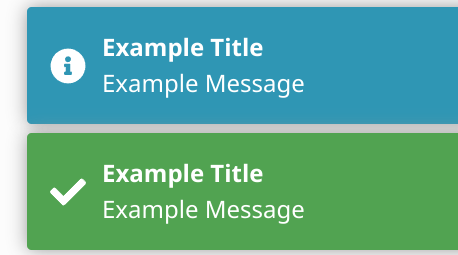
\includegraphics[width=0.9\linewidth]{diagrams/success-info.png}
    \caption{Info/Success diagrams}
    \label{fig:sub2}%
  \end{subfigure}
  \begin{subfigure}{.45\textwidth}
    \centering
    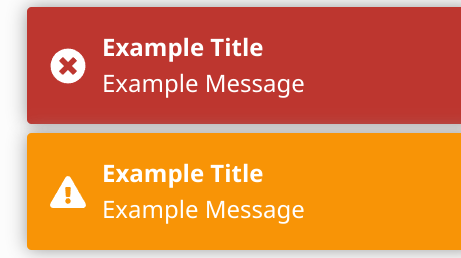
\includegraphics[width=0.9\linewidth]{diagrams/warning-error.png}
    \caption{Error/Warning diagrams}
    \label{fig:sub1}
  \end{subfigure}%
  \caption{Toastr diagrams}
  \label{fig:figma3}
\end{figure}


\section{Code}

\subsection{User login and registration}
\subsubsection{Sequence Diagrams}

\paragraph{Login.}
It follows a discussion of the sequence of steps required for user
authentication. This is depicted in Diagram \ref{fig:login}.

\begin{enumerate}
  \item User. The user inserts the credentials into the browser.
  \item Frontend (Angular). Makes an http authentication request. The http
    service used to perform the request is provided by the Angular framework.
  \item Backend (ExpressJS). The server queries MongoDB for user's credentials
    and verifies them against the provided ones and as a result returns success
    or failure.
  \item Database (MongoDB). Used to store user authentication information. The
    data is encrypted using bcrypt as explained in Section \ref{sec:bcrypt}.
    This library is used in order to provide additional security against Rainbow
    Dictionary Attacks \autocite{wiki:rainbow-attacks}.
\end{enumerate}

\begin{figure}[h]
  \centering
  \includesvg{diagrams/svgs/login-sequence-diagram}
  \caption{Login Sequence Diagram}
  \label{fig:login}
\end{figure}


\begin{figure}[h]
  \centering
  \includesvg{diagrams/svgs/register-sequence-diagram}
  \caption{Registration Sequence Diagram}
  \label{fig:register}
\end{figure}

\paragraph{Registration.}
Moreover, Figure \ref{fig:register} depicts the registration process, which is
very similar to the diagram shown in Figure \ref{fig:login}. The entities
described in the previous list apply here as well.

These sequence diagrams illustrate a simplified login/registration process,
however the actual implementation varies and will also involve error handling,
encryption of data, generation of the JSON Web Token, as it was discussed in
Section \ref{sec:bcrypt} and \ref{sec:jsonwebtoken} respectively.


\subsubsection{Class Diagrams}
Figures \ref{fig:class-user} and \ref{fig:class-dashboard} show two class
diagrams which depict the relationship between the different modules and classes
across the two most important modules of the application: the User and the
Dashboard respectively.

There are similarities between the two modules. Both of them make use of a base
module which encompasses information that is reusable around the entire
application. This module is extensively shared across and enables information
such as the dashboard, guards, models, toolbar or services to exist in only one
place. This kind of modularity provides advantages in terms of flexibility,
scalability and maintainability of existing code as it was shown by the two
diagrams that were recently mentioned.

\paragraph{User Module}
In Figure \ref{fig:class-user}, the structure of the project becomes clearer.
Firstly, there is the {\em{UserModule}} which spawns the entire chain of
dependencies. There are two high level components which spring from it
({\em{RegistrationComponent}} and {\em{LoginComponent}}), which in turn make use
of a shared {\em{UserService}}, residing in the {\em{BaseModule}}. Moreover,
these components make use of DTOs\footnote{DTO - Data Transfer Object} to
manipulate data around, making use of Typescript's strong typed system.


\begin{figure}[h]
  \centering 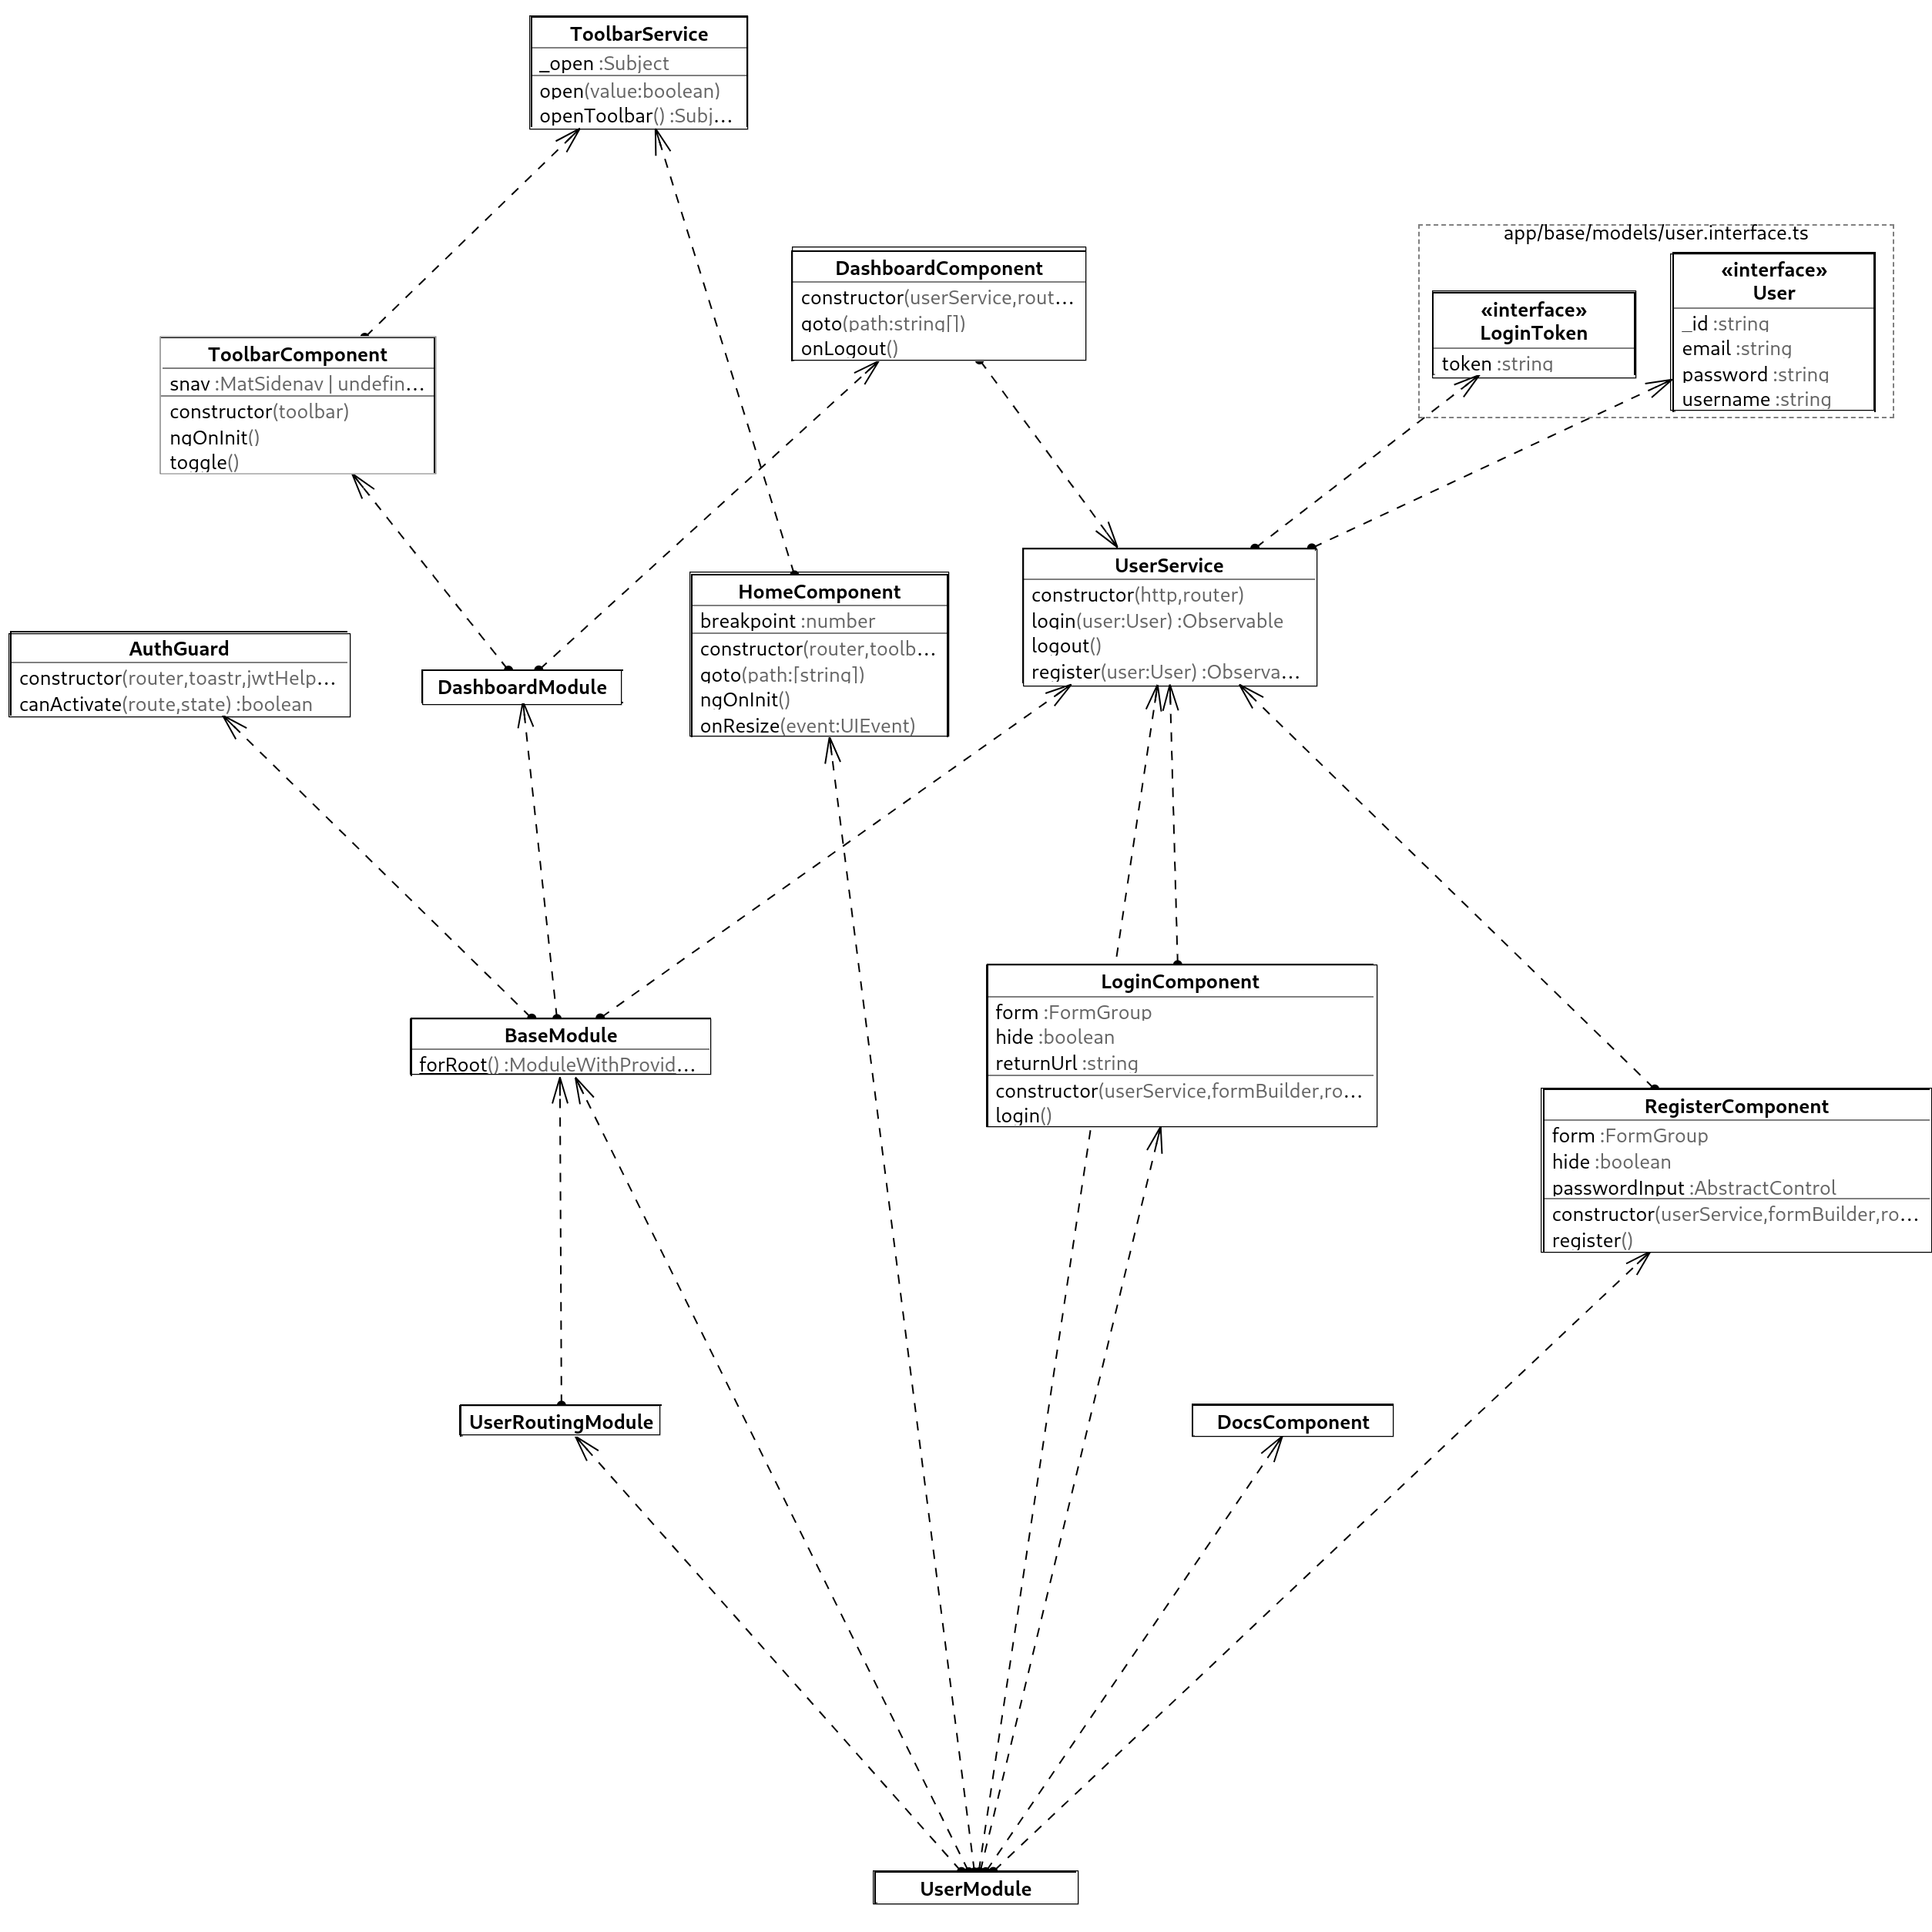
\includegraphics[scale=0.15]{diagrams/client-side_diagram1.png}
  \caption{Angular User module class diagram}
  \label{fig:class-user}
\end{figure}
\begin{figure}[h]
  \centering
  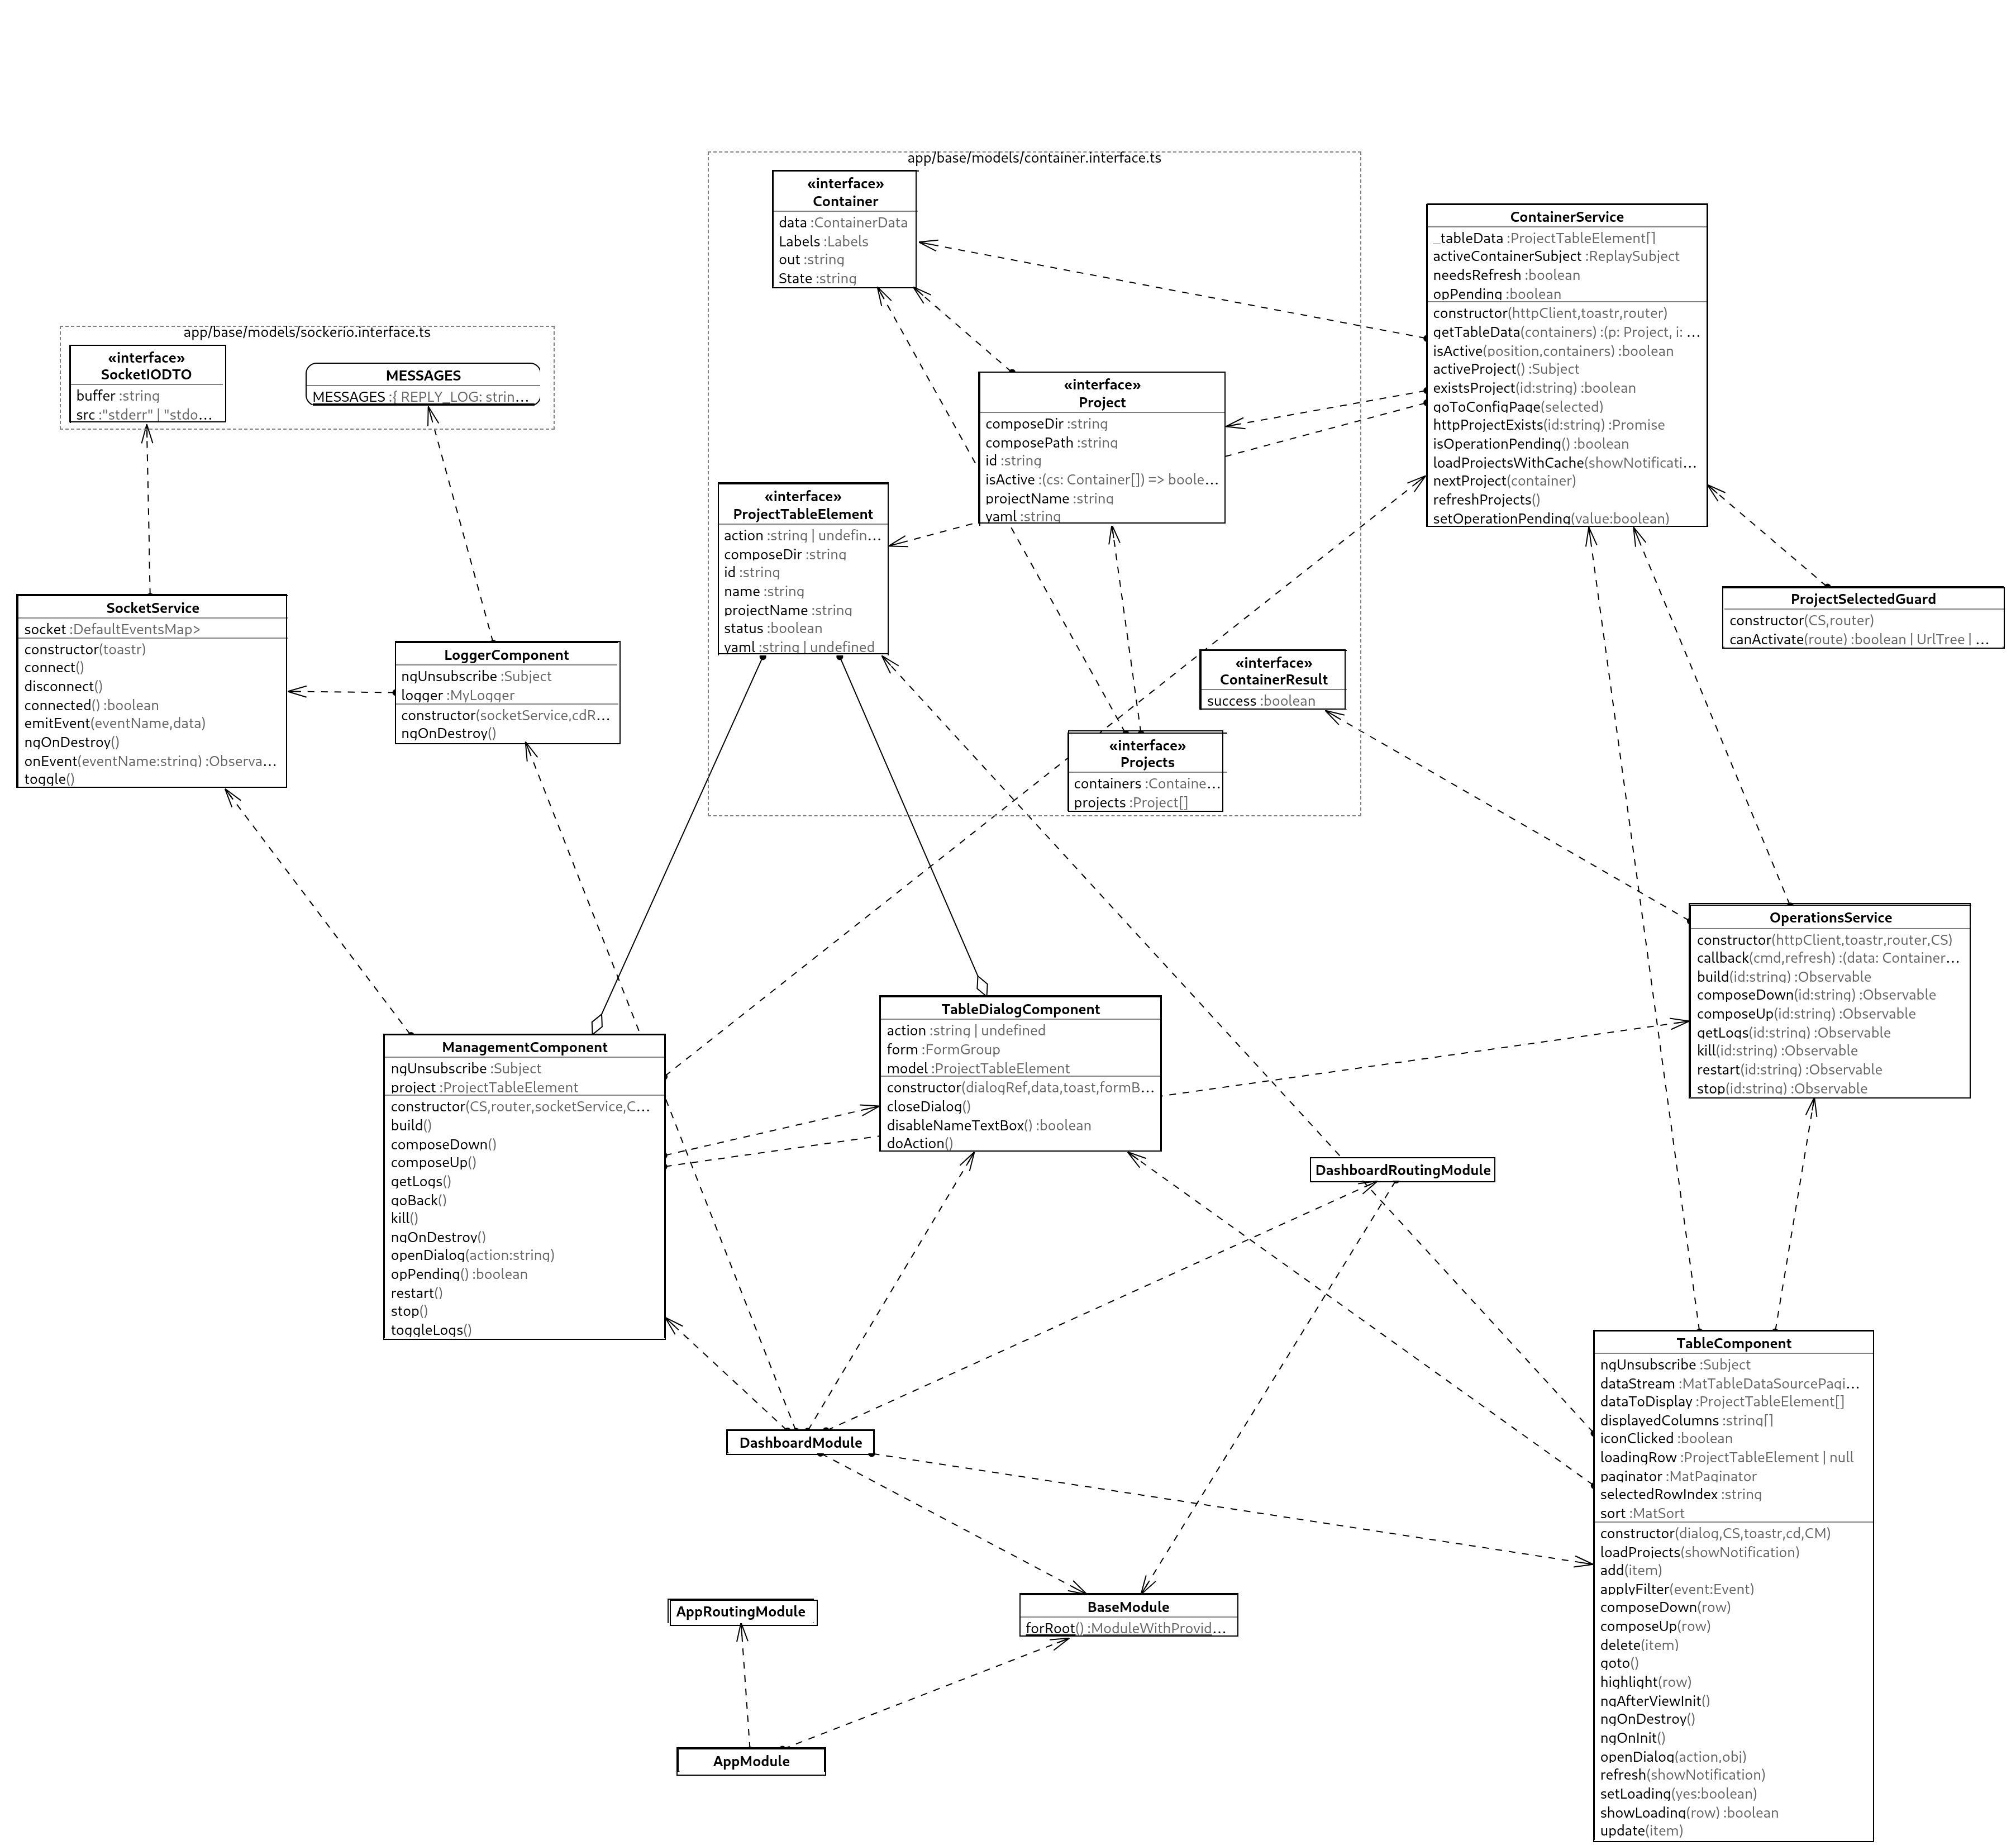
\includegraphics[scale=0.1]{diagrams/client-side_diagram2.png}
  \caption{Angular Dashboard module class diagram}
  \label{fig:class-dashboard}
\end{figure}

\paragraph{Dashboard Module}
On the other hand, it follows of description of Figure
\ref{fig:class-dashboard}. The dashboard module is slightly more complex, since
the processes which it must describe are more involved. However, the general
layout described in the previous paragraph still holds. The module can be
described through three components:

\begin{enumerate}
\item ManagementComponent. It contains the functionality related to managing a
  selected projects. This includes commands such as building, starting or
  closing all services within a project.
\item TableComponent. It displays the projects that were detected inside the
  projects' root directory ({\em{server-side/docker-projects}}) as a Material
  table. This page makes use of the modal defined in TableDialogComponent.
\item TableDialogComponent. Used to display information about a specific
  project. It aids usability as the application provides a quick way of
  inspecting a specific project's build instructions.
\end{enumerate}


\subsection{Back-end Code organization}
As it is shown in Figure \ref{fig:backendcode}, the back-end is organized around
the MVC pattern and some of its features and advantages were described in
Section \ref{sec:mvc-design}.

\begin{itemize}
\item Project's root contains configuration files such as \textbf{package.json}
  to determine project dependencies and the \textbf{.gitignore} file.
\item The root directory contains a Dockerfile which is used to create an image
  which is subsequently deployed to Docker Hub.
\item The code is organized under the MVC pattern and is organized as follows:
  \begin{itemize}
  \item \textbf{controllers}: define logic for handling HTTP requests and
    responses.
  \item \textbf{models}: define the data structures and schemas for MongoDB
    documents.
  \item \textbf{routes}: define API routes and link them to corresponding
    controllers.
  \item \textbf{services}: reusable code across the different files.
  \end{itemize}
\end{itemize}




\begin{figure}
  \centering
  \begin{forest}
    pic dir tree,
    for descendants={% folder icons by default; override using file for file icons
      directory,
    },
    draw linear split tree,
    to be continued/.style 2 args={
      dots below={#2},
      arrow to next tree,
    },
    [server-side
      [bin
        [
          \fname{www.js}{start-up script}, file
        ]
      ],
      [\fname{config}{env. variables}
        [config.js, file]
      ],
      [controllers
        [container.controller.js, file]
        [user.controller.js, file]
      ]
      [\fname{Dockerfile}{\quad\quad docker image}, file]
      [\fname{docker-projects}{\quad\quad\quad\quad\quad projects' root}]
      [models
        [container.model.js, file]
        [project.model.js, file, split here]
        [user.model.js, file]
      ]
      [node\_modules]
      [\fname{package.json}{\quad\quad\quad deps}, file]
      [routes
        [container.js, file]
        [user.js, file]
      ]
      [services
        [dockerAdapter.service.js, file]
        [fileSystem.service.js, file]
        [socketIO.service.js, file]
      ]
    ]
  \end{forest}
  \caption{Server side code organization}\label{fig:backendcode}
\end{figure}


\subsection{Frontend code organization}

The folder \textbf{frontend} holds all client side Angular code, is shown in
Figure \ref{fig:clientside} and is organized as follows:

\begin{itemize}
  \item \textbf{Root} directory contains:
  \begin{itemize}
  \item \textbf{angular.json} configuration file for Angular
  \item \textbf{Dockerfile} for creating an image which is used for deployment
    via Docker Hub
  \item \textbf{package.json} used to define NodeJS dependencies.
  \end{itemize}
  \item \textbf{config} folder contains the environment variables used for
    MongoDB, encryption, server and socket IO endpoints, etc.
  \item \textbf{src} directory contains the component that bootstraps the
    application, all other components spawn from here.
  \item \textbf{src/base} contains components, services, models and guards that
    are shared across the whole application. This folder is composed of entities
    that do not partake to some specific feature but are shared across different
    areas of the application. This could be the registration or login features
    or the management of containers.
    \begin{itemize}
    \item \textbf{Dashboard}: contains left hand side menu which can be toggled on and
      off.
    \item \textbf{Authentication Guard}: ensures that the user is logged in prior to
      accessing specific resources.
    \item \textbf{Models}: models used for hard typing data that arrives from the server.
    \item \textbf{Services}: needed to share data across components.
    \item \textbf{Toolbar}: this is the bar from the top area of the screen. Used to
      toggle the dashboard navigation list.
    \end{itemize}
  \item \textbf{src/components}: define the main features: login/registration,
    management of the containers, home page and documentation page.
\end{itemize}




\begin{figure}
  \centering
  \begin{forest}
    pic dir tree,
    for descendants={% folder icons by default; override using file for file icons
      directory,
    },
    draw linear split tree,
    to be continued/.style 2 args={
      dots below={#2},
      arrow to next tree,
    },
    [client-side
      [\fname{angular.json}{}, file]
      [config
        [\fname{environment.ts}{}, file]
        [\fname{environment.docker.ts}{}, file]
      ]
      [\fname{Dockerfile}{}, file]
      [node\_modules
      ]
      [\fname{package.json}{\quad\quad\quad 3rd party deps}, file]
      [\fname{package\_lock.json}{}, file]
      [src
        [\fname{app.component.ts}{}, file]
        [\fname{app.component.html}{}, file]
        [\fname{app.component.css}{}, file]
        [\fname{app.module.ts}{}, file]
        [\fname{app-routing.module.ts}{}, file]
        [base
          [base.module.ts, file]
          [dashboard
            [..., file]
            [\fname{dashboard.module.ts}{}]
          ]
          [footer
            [..., file]
          ]
          [guards
            %[..., file]
          ]
          [models
            %[..., file]
          ]
          [services
            [\fname{operations.service.ts}{}, file]
            [\fname{container.service.ts}{}, file]
            [\fname{socket.service.ts}{}, file]
            [\fname{user.service.ts}{}, file]
          ]
          [toolbar, split here
            %[..., file]
          ]
        ]
        [components
          [dashboard
            [dashboard.module.ts, file]
            [dashboard-routing.module.ts, file]
            [home
              [\fname{...}{}, file]
            ]
            [logger
              [\fname{...}{}, file]
            ]
            [management
            [\fname{...}{}, file]
            ]
            [table
              [\fname{...}{}, file]
            ]
            [table-dialog
              [\fname{...}{}, file]
            ]
          ]
          [user
            [login]
            [register]
            [user.module.ts, file]
            [user-routing.module.ts, file]
          ]
        ]
        [assets
          [icons
            [\fname{...}{}, file]
          ]
        ]
        [\fname{main.ts}{}, file]
        [\fname{styles.scss}{}, file]
      ]
      [\fname{tsconfig.app.json}{}, file]
      [\fname{tsconfig.json}{}, file]
    ]
  \end{forest}
  \caption{Client side code organization}\label{fig:clientside}
\end{figure}





\section{Test}
As far as testing goes, there were used two techniques. First one entails the
creation of prototypes using Figma at the beginning of the project and the other
one involved using questionnaires to gauge the robustness of the final result
after the project has been developed.

\subsection{Figma}

\paragraph{What is Figma?}
It is a collaborative web application for interface design. The feature set of
Figma focuses on user interface and user experience design, with an emphasis on
real-time collaboration, utilising a variety of vector graphics editor and
prototyping tools \autocite{wiki:figma}.


Some of its key features include \textbf{Vector Editing}, \textbf{Prototyping},
\textbf{Component Libraries} and \textbf{Plug-ins}, all of which were used to
some degree.


\paragraph{Figma as a design tool.}
Figma was the main technology used for prototyping the system. As a consequence
of creating user stories and design tasks which were discussed in Sections
\ref{sec:stories} and \ref{sec:tasks}, there were made multiple Figma diagrams,
which drove the development of the application. There were times when initial
sketches did not make it into the final version (i.e. design decisions which
were subsequently abandoned) and as a result Figma proved to be a useful tool
for planning the application. Mock-ups were used for assessing the user
experience, proving to have a significant impact into how the final result was
tailored.


The Figma mock-ups can be found online\footnote{The Figma project together with
all sketches used to devise the mock-ups can be found
\href{https://www.figma.com/file/TGgkRNt5faxYmILkp60JdN/Docker-UI?type=design&node-id=0-1&mode=design&t=rZRXwLEom6yfP9AU-0}{here.}}.
However, I will display the main diagrams in this document to illustrate and
comment upon some of the relevant design decisions. The diagrams can be seen at
Figures \ref{fig:figma1}, \ref{fig:figma2} and \ref{fig:figma3}.


\begin{figure}[h]
  \centering
  \begin{subfigure}{.5\textwidth}
    \centering
    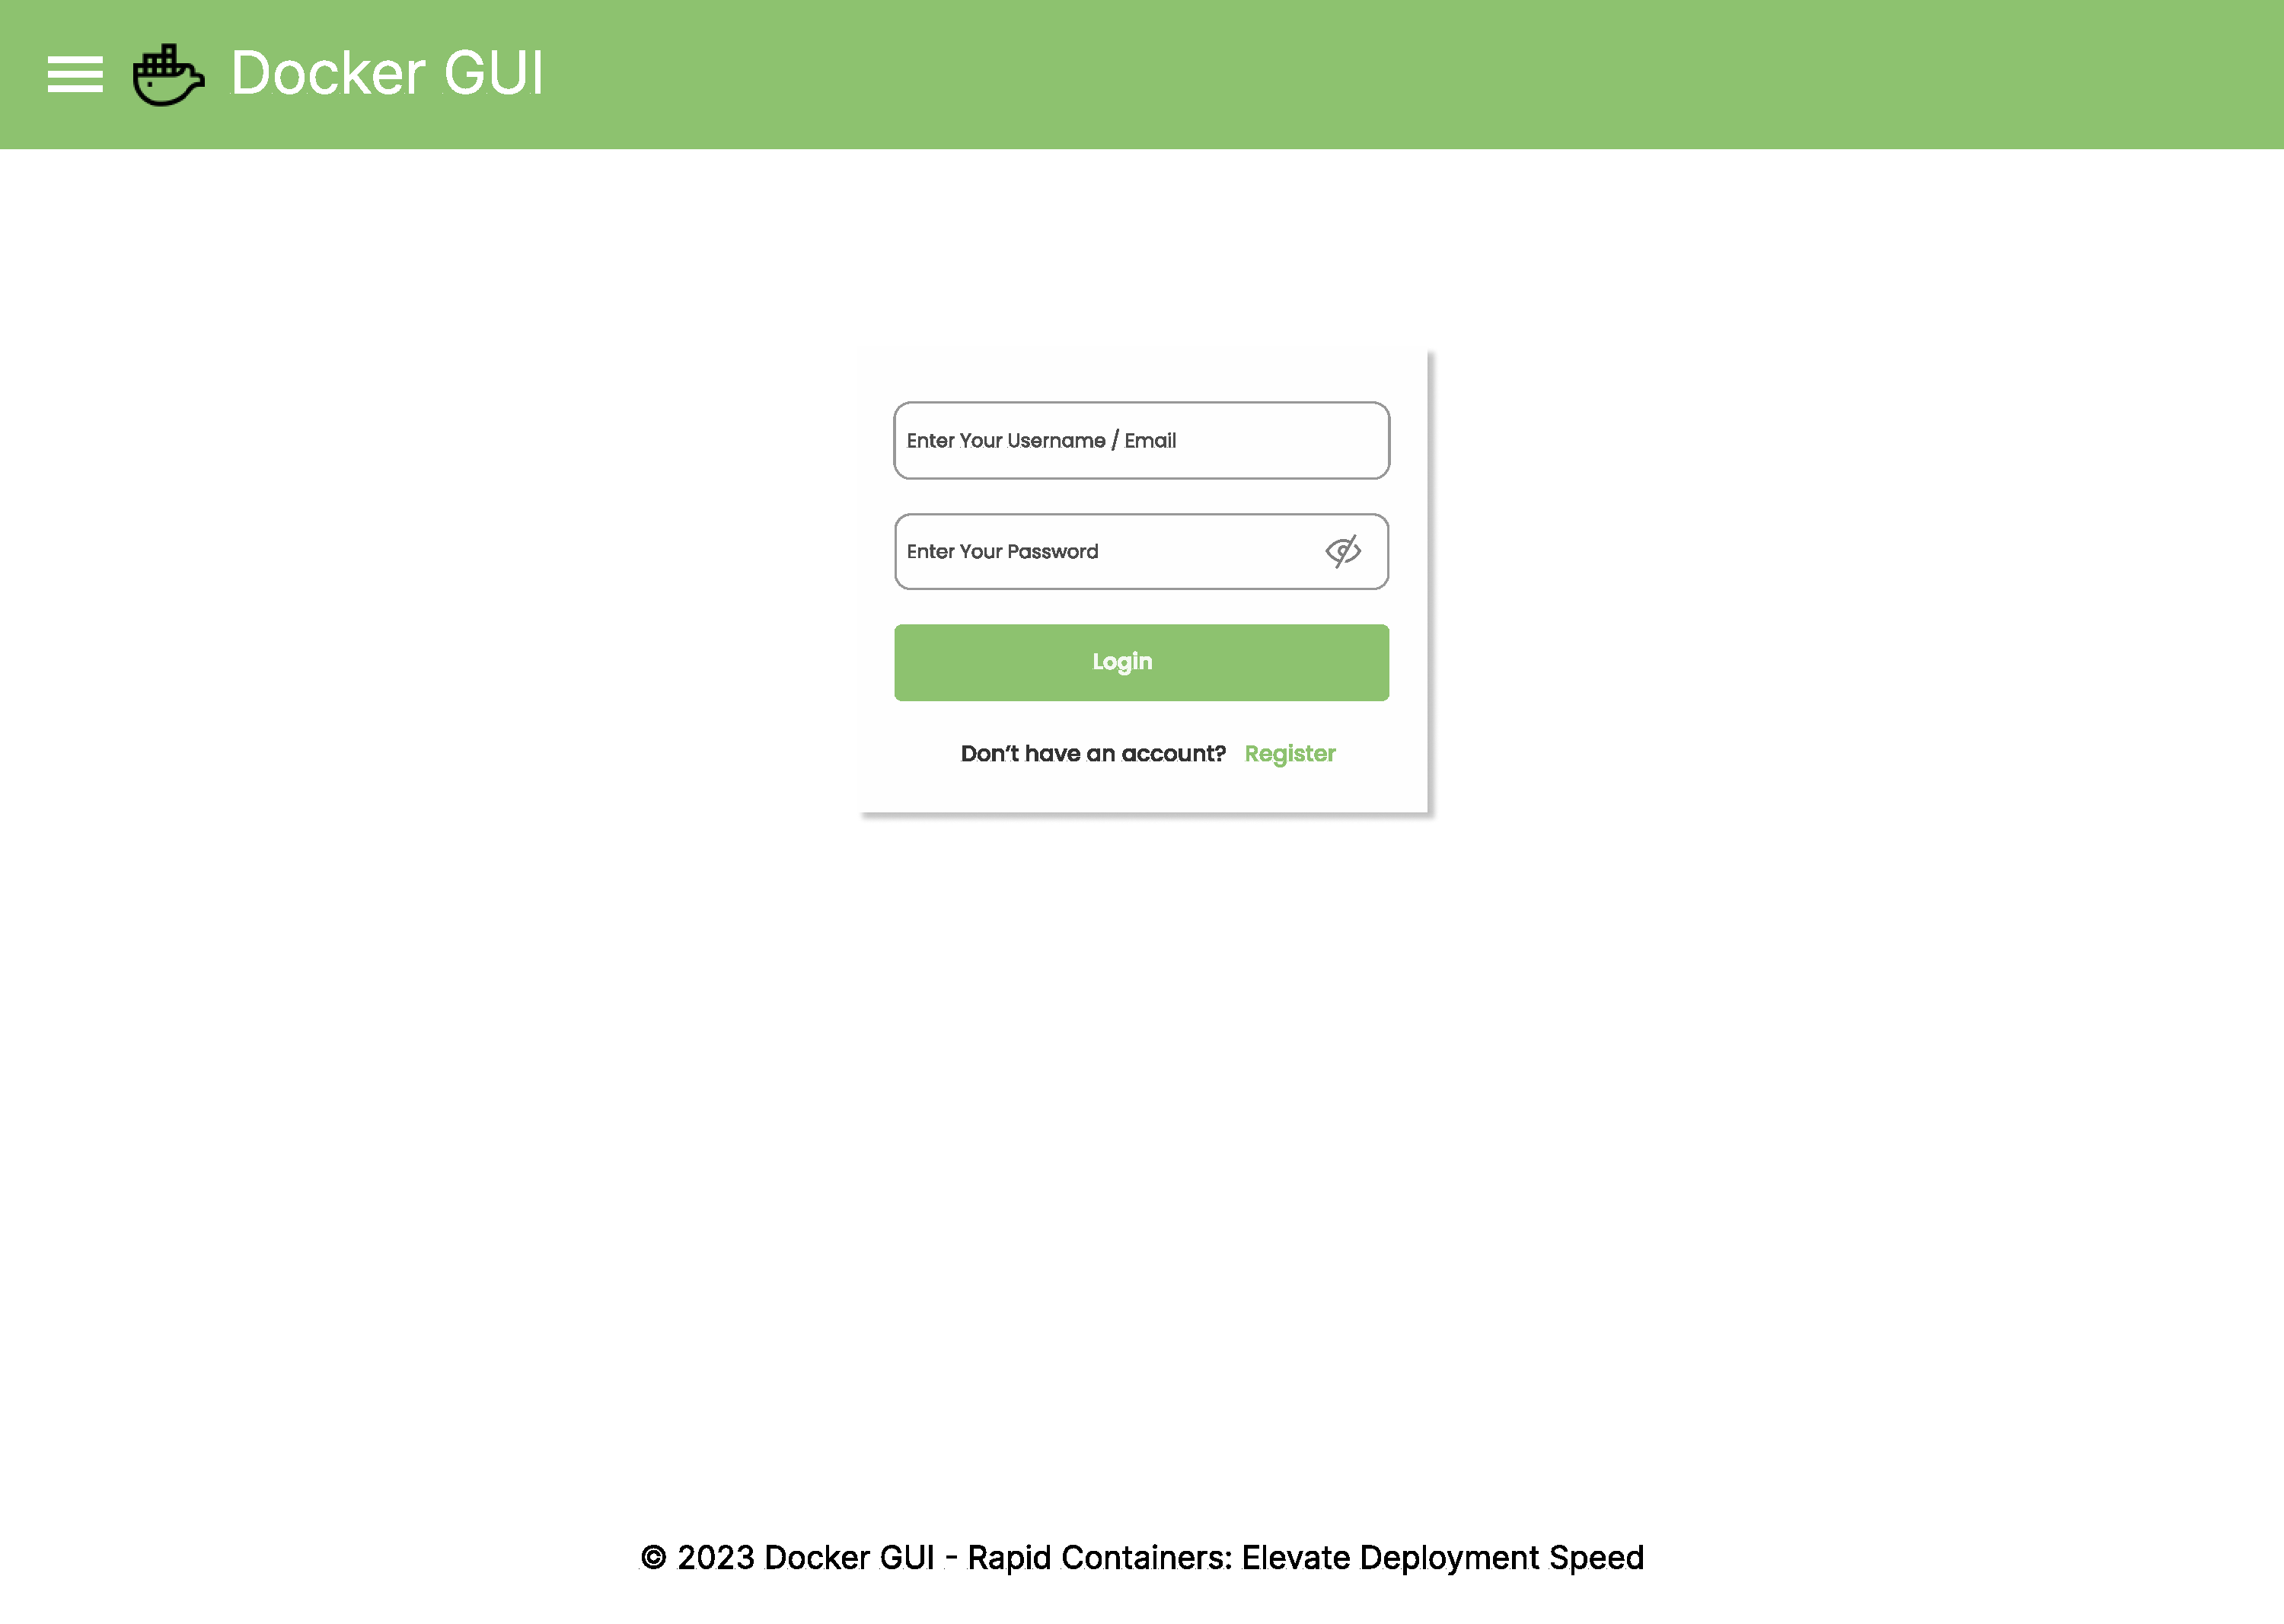
\includegraphics[width=.95\linewidth]{diagrams/1.login.pdf}
    \caption{http://localhost:4200/login}
    \label{fig:sub1}
  \end{subfigure}%
  \begin{subfigure}{.5\textwidth}
    \centering
    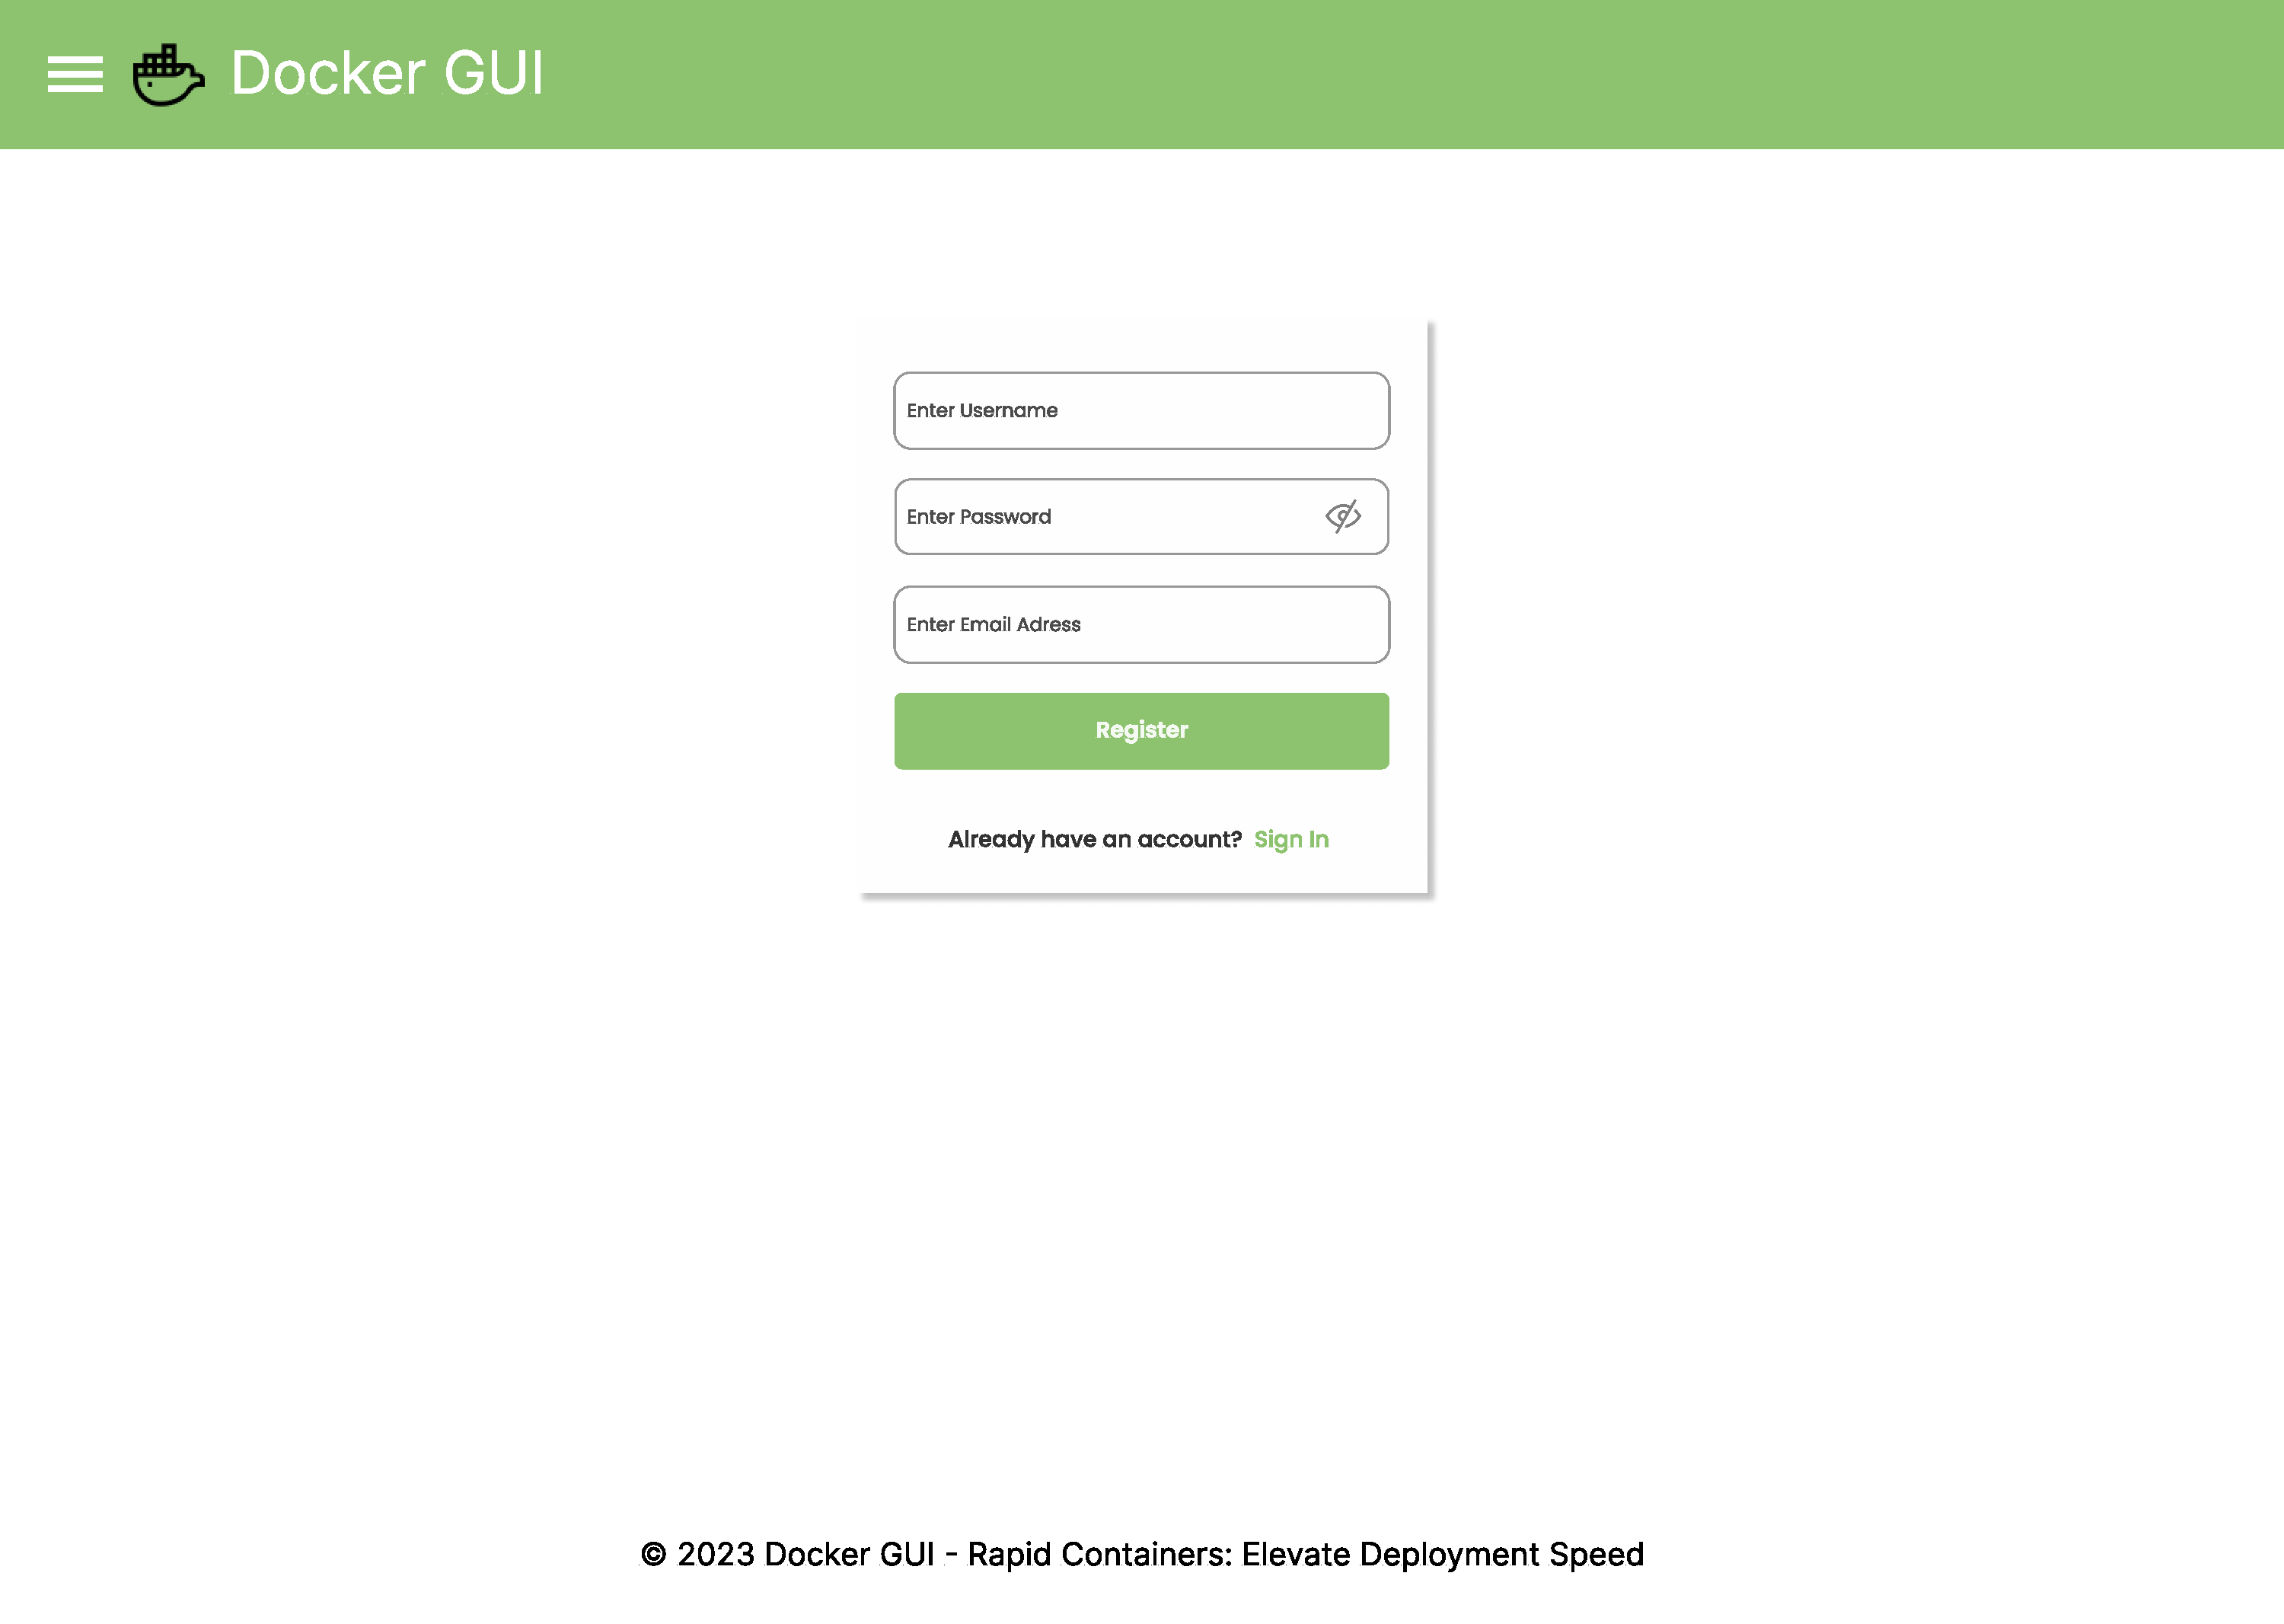
\includegraphics[width=.95\linewidth]{diagrams/1.registration.pdf}
    \caption{http://localhost:4200/register}
    \label{fig:sub2}
  \end{subfigure}
  \caption{Login and Registration pages}
  \label{fig:figma1}
\end{figure}

\begin{figure}[h]
  \centering
  \begin{subfigure}{.5\textwidth}
    \centering
    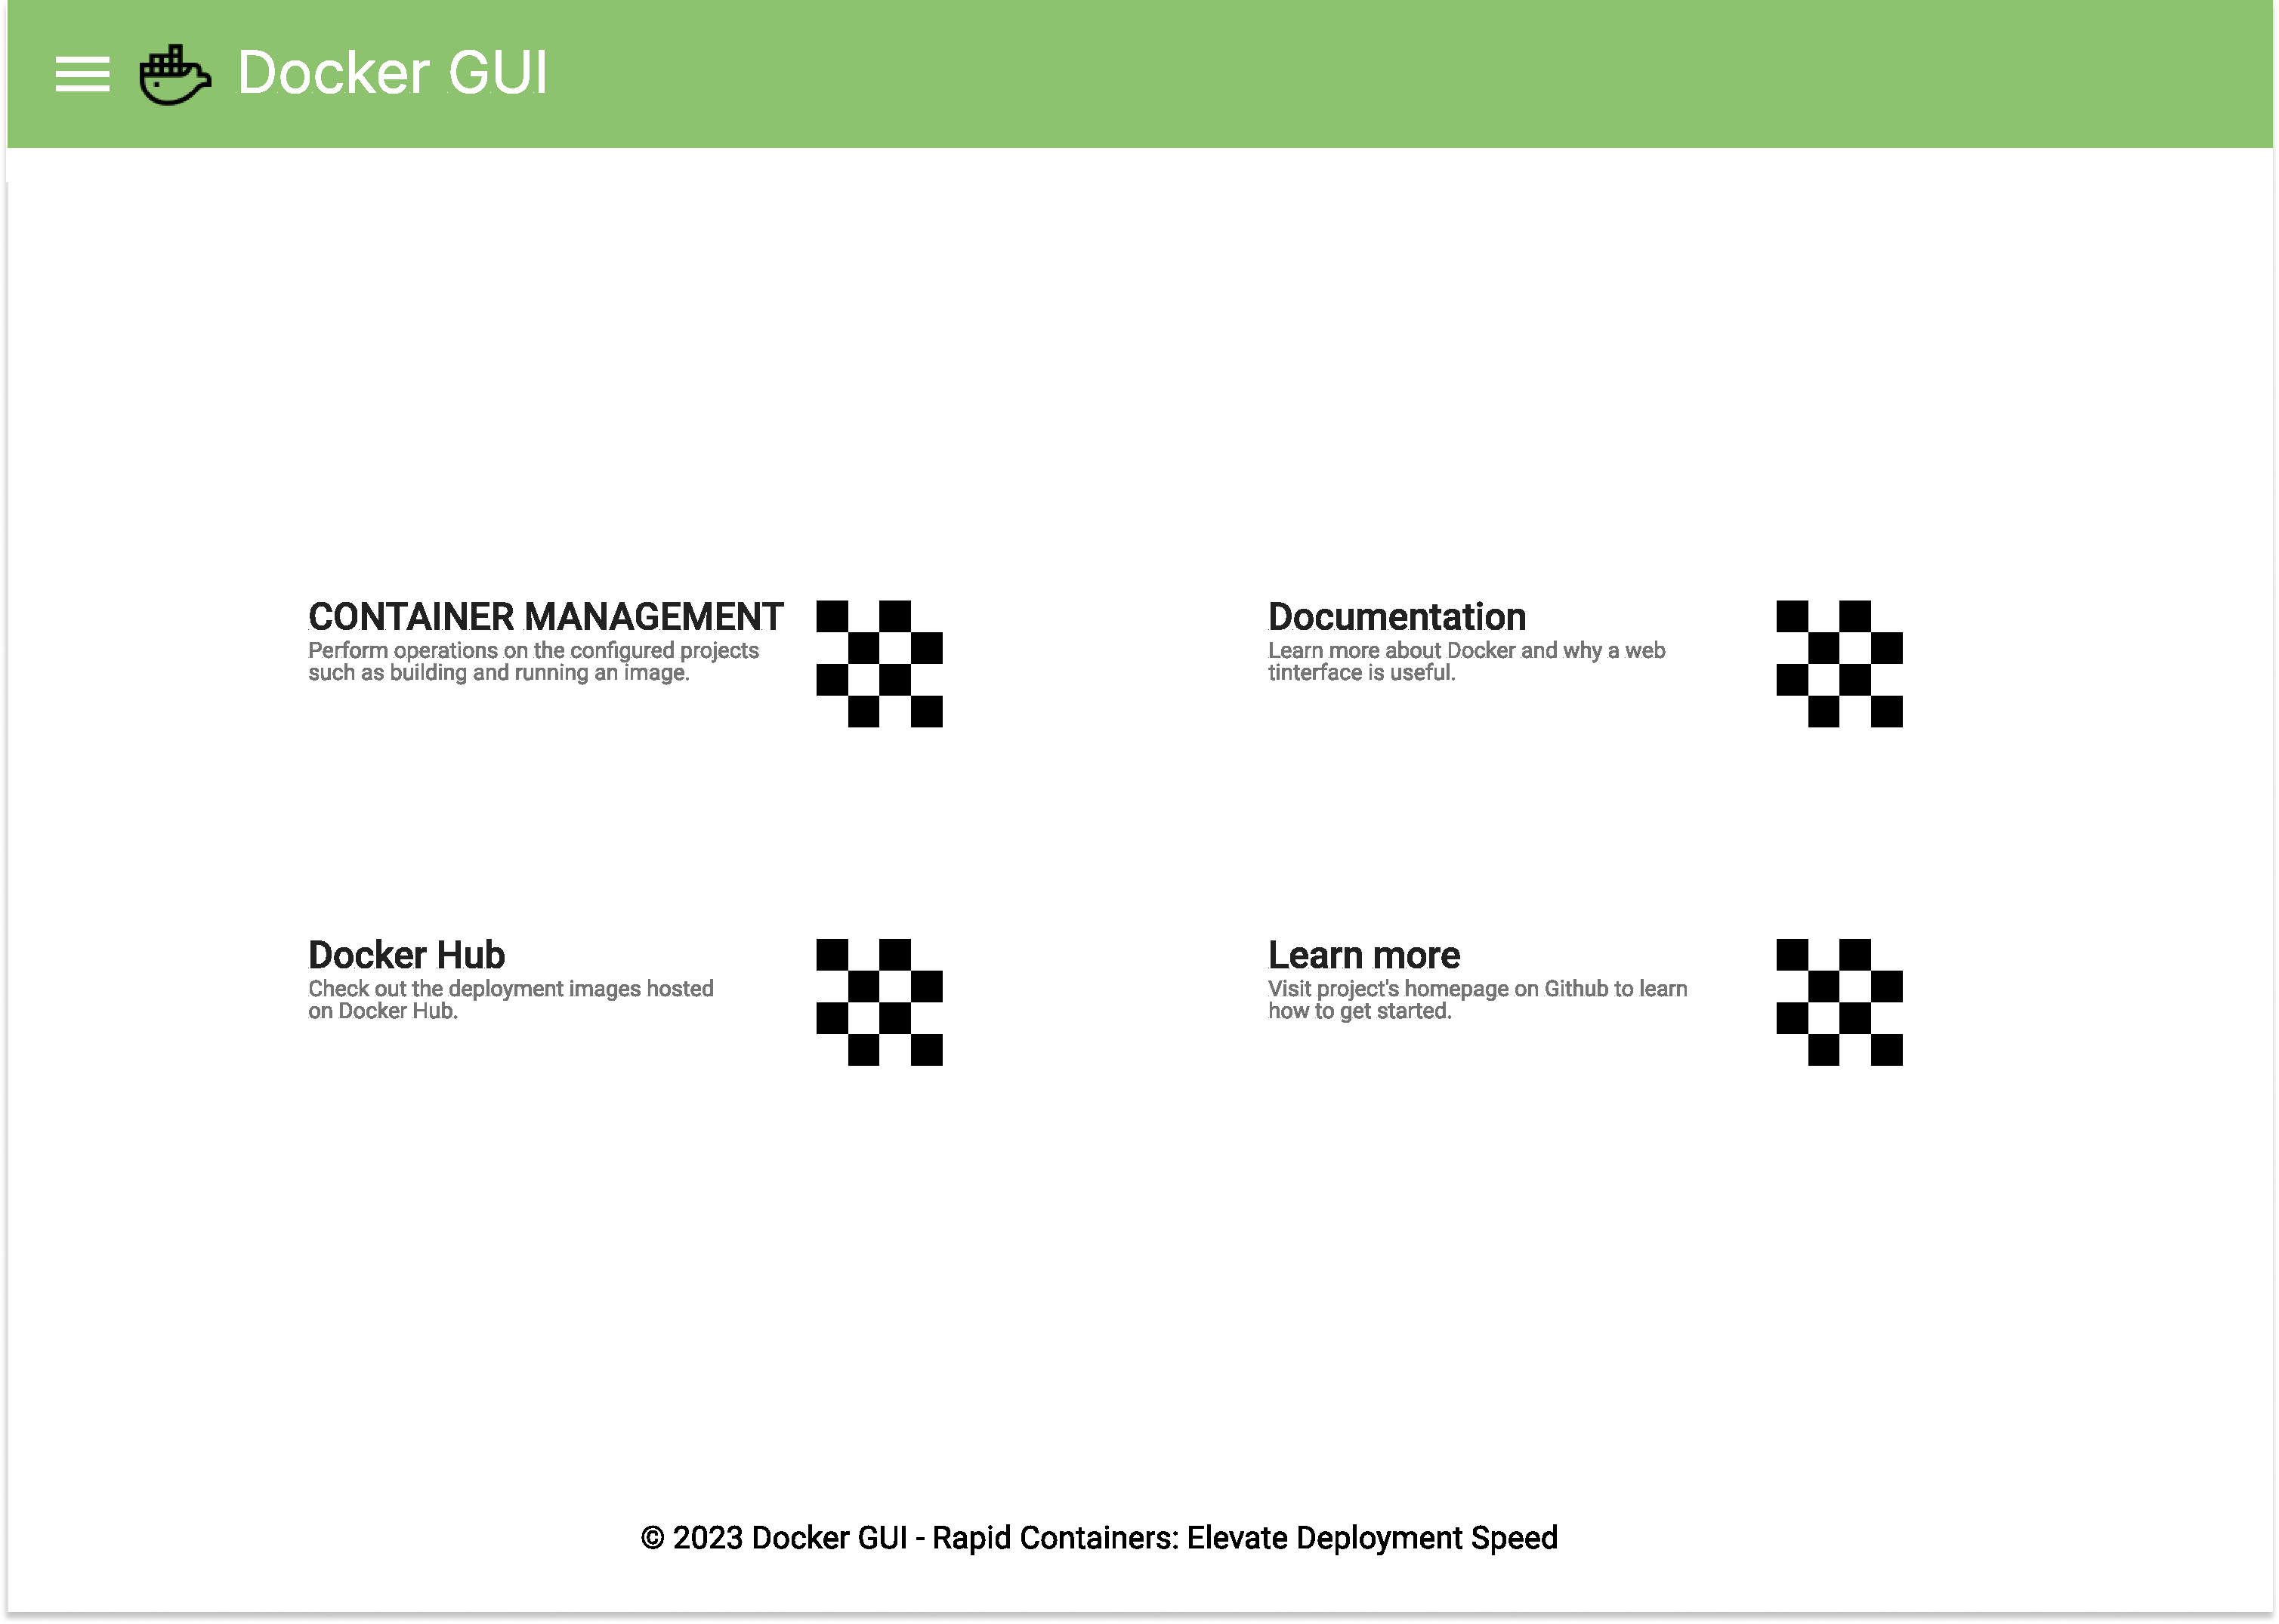
\includegraphics[width=.95\linewidth]{diagrams/2.homepage.pdf}
    \caption{http://localhost:4200/dashboard}
    \label{fig:sub1}
  \end{subfigure}%
  \begin{subfigure}{.5\textwidth}
    \centering
    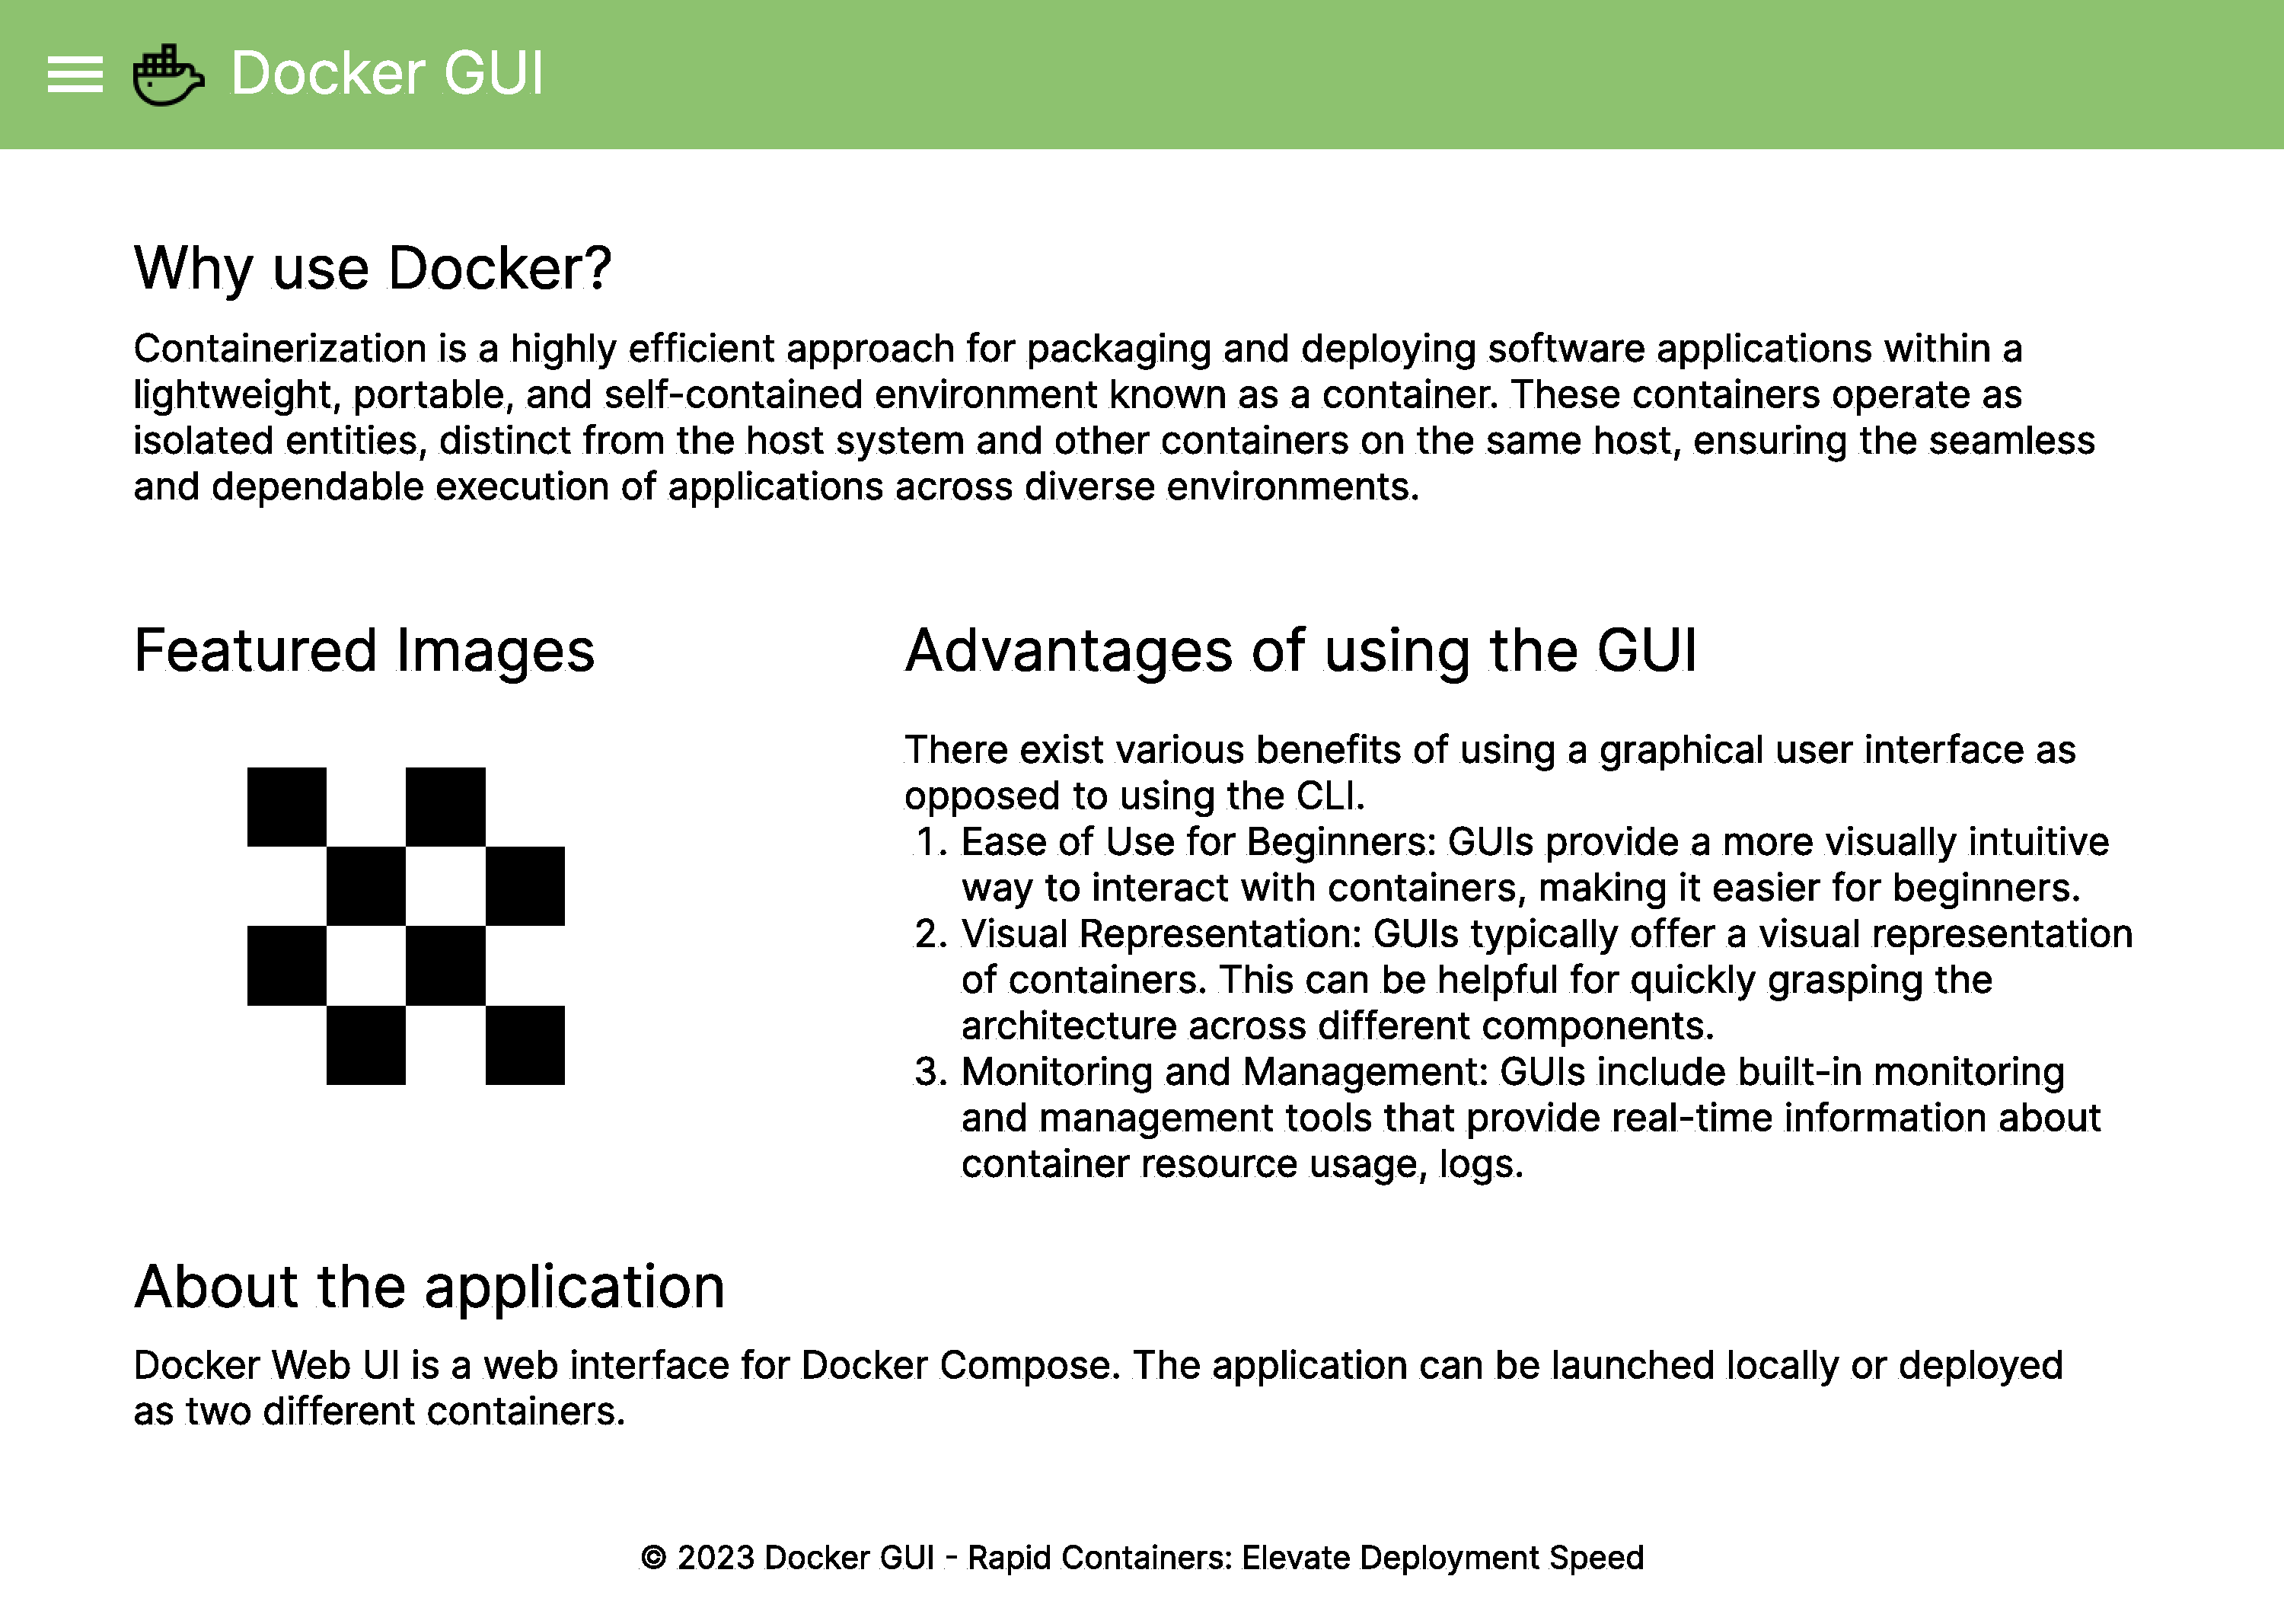
\includegraphics[width=.95\linewidth]{diagrams/5.docs.pdf}
    \caption{http://localhost:4200/dashboard/docs}
    \label{fig:sub2}
  \end{subfigure}
  \caption{Home and Documentation pages}
  \label{fig:figma2}
\end{figure}

\begin{figure}[h]
  \centering
  \begin{subfigure}{.5\textwidth}
    \centering
    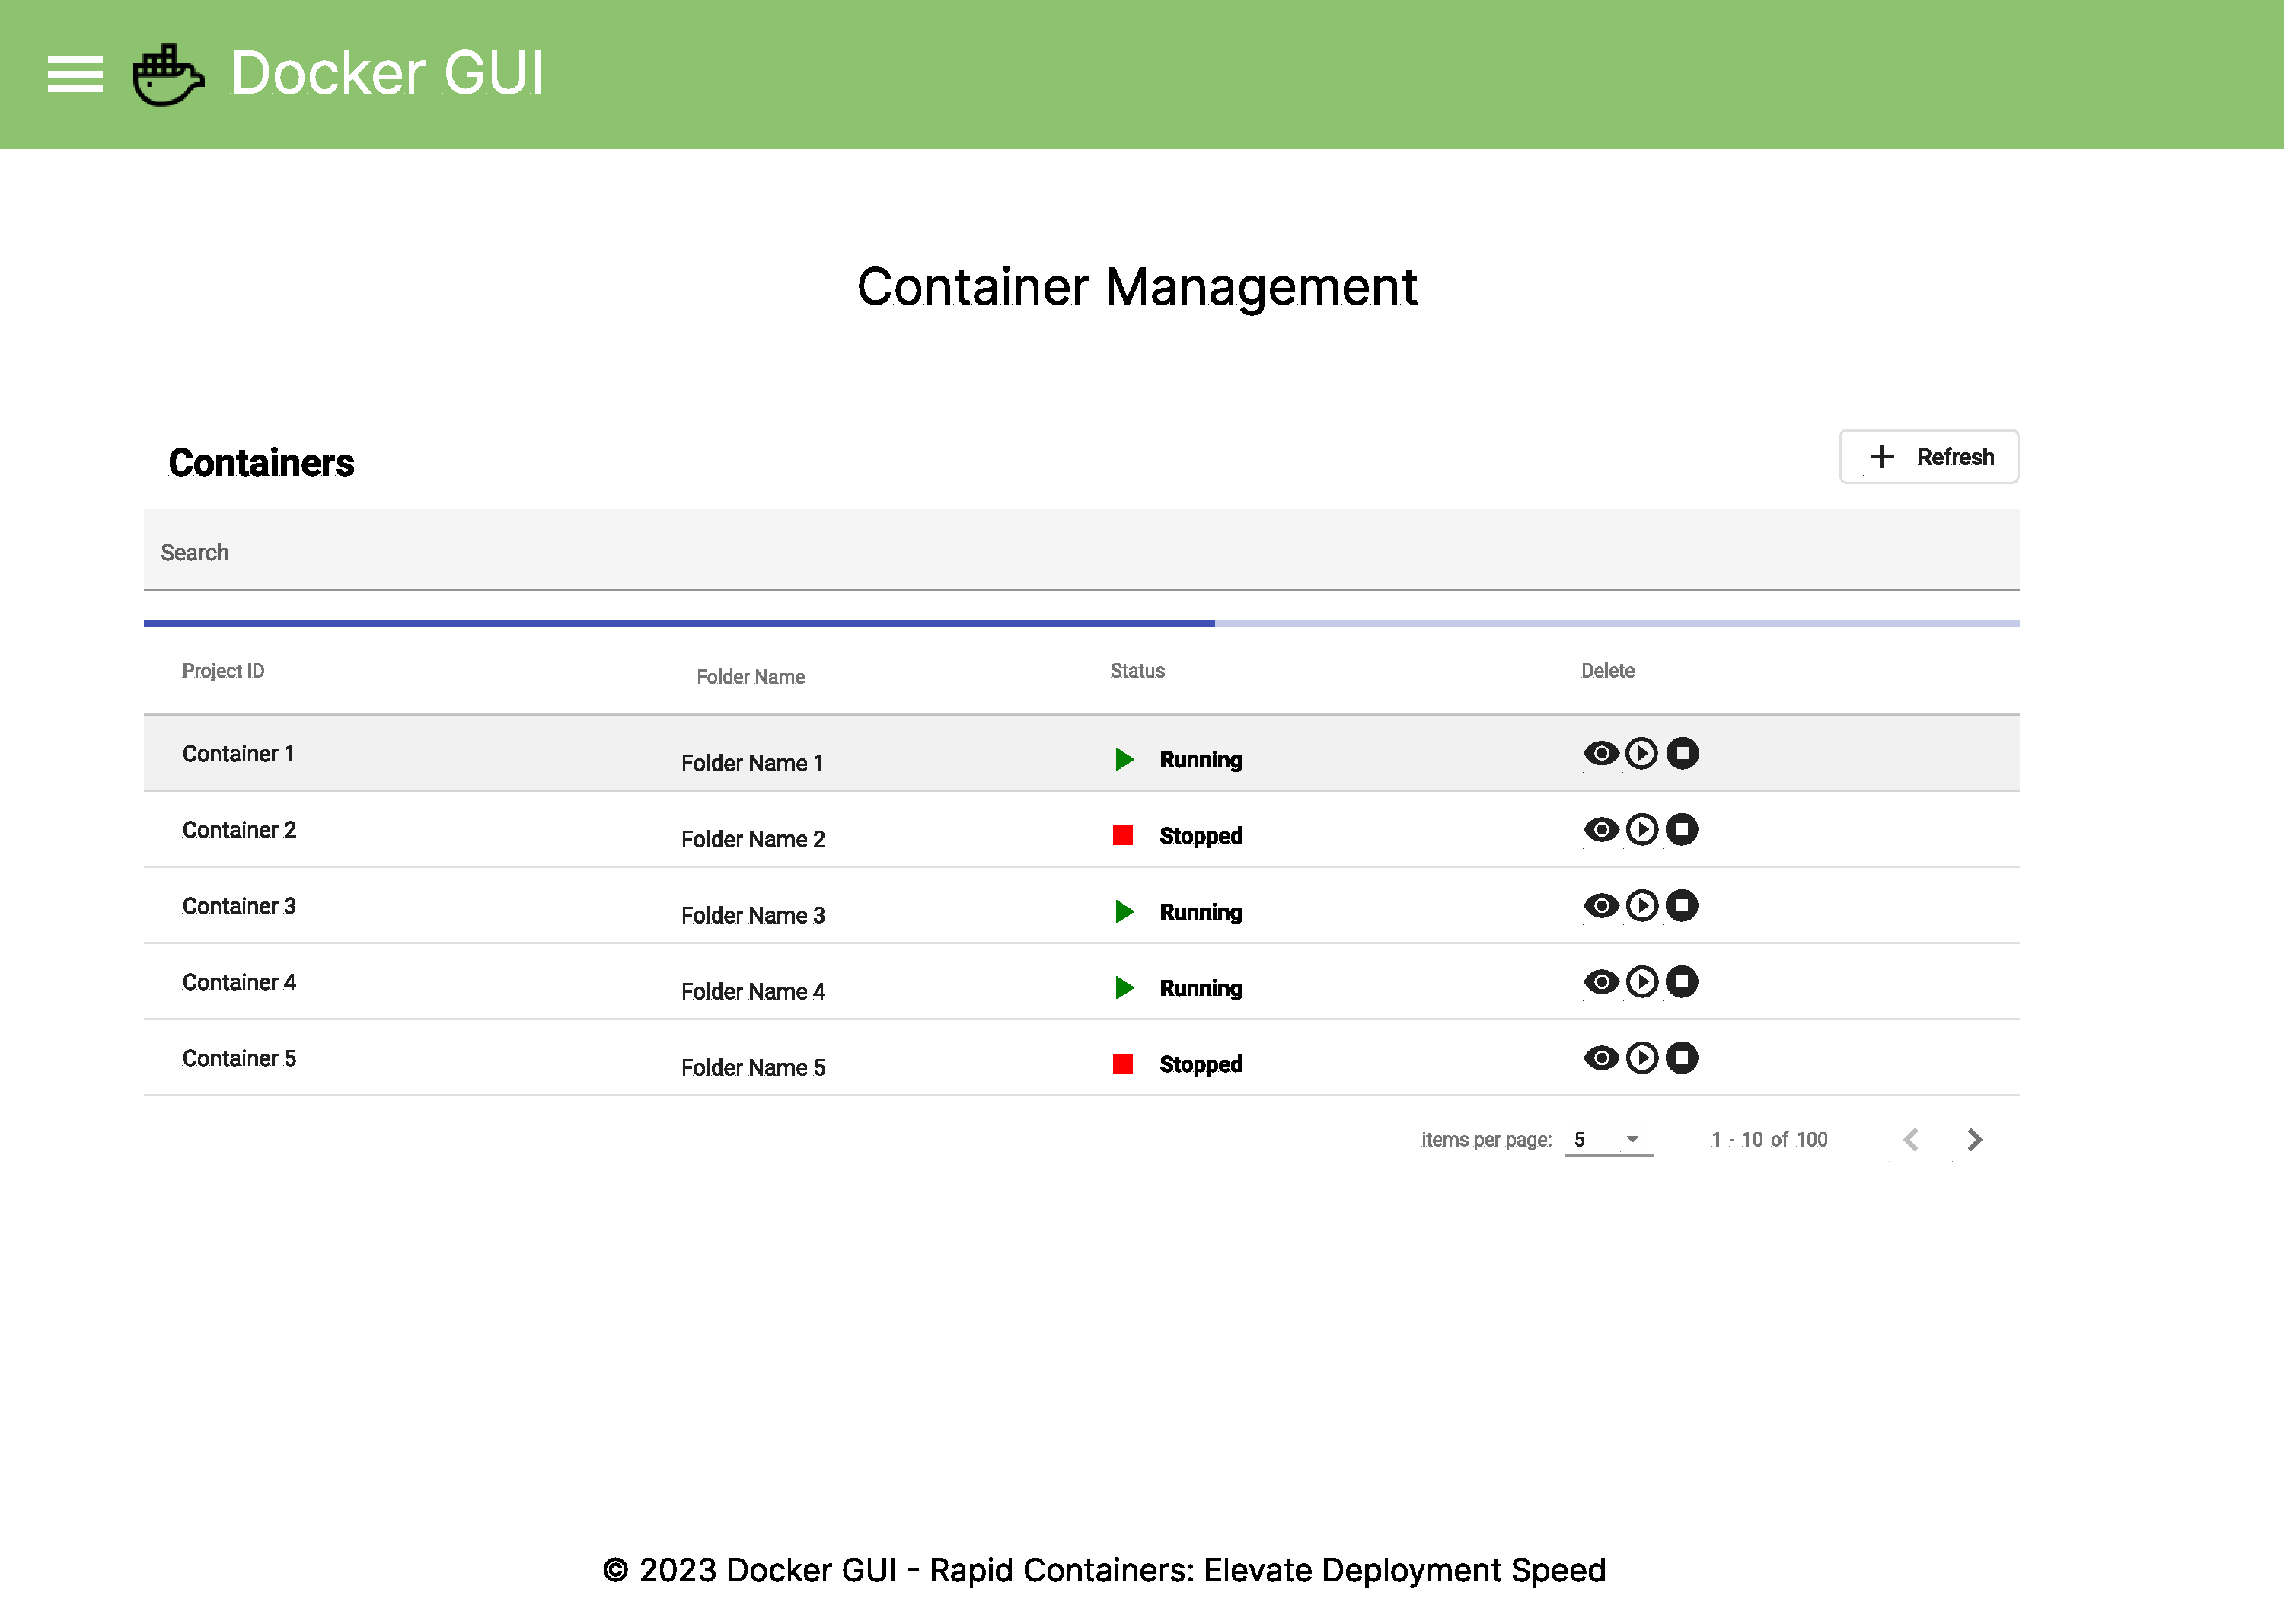
\includegraphics[width=0.95\linewidth]{diagrams/3.container.pdf}
    \caption{http://localhost:4200/dashboard/containers}
    \label{fig:sub1}
  \end{subfigure}%
  \begin{subfigure}{.5\textwidth}
    \centering
    \includegraphics[width=0.95\linewidth]{diagrams/4.management.pdf}
    \caption{http://localhost:4200/dashboard/containers/<id>}
    \label{fig:sub2}
  \end{subfigure}
  \caption{Container and Container Management pages}
  \label{fig:figma3}
\end{figure}


\subsubsection{Benefits of using Figma}
As it has been suggested, developing the prototypes helped highlight subpar
design decisions which were improved timely, in essence gauging relevant areas
of improvement by creating a tangible high level description of the application.
In essence, it helped guide important decisions before losing sight of the
bigger picture by delving into the particularities of how application details
shall be developed.

In particular, initially the login/registration pages were designed as it is
shown in Figure \ref{fig:login-registration-old} but the final implementation is
displayed in Figure \ref{fig:figma1}. Essentially, Figma helped individuate
cluttered areas, which represented areas of improvement (i.e. the brightness and
contrast of the registration page were particularly high) and were taken care of
by making modifications such as changing the background color or adjusting the
size of the widgets used for login/registration.

Similarly, the logger's display area (Figure b of
\ref{fig:login-registration-old}), was changed as it was initially too cluttered
and as a result was moved to its own page. The separation enhanced and hopefully
made for a more robust and intuitive browsing experience.

\begin{figure}[h]
  \centering
  \begin{subfigure}{.5\textwidth}
    \centering
    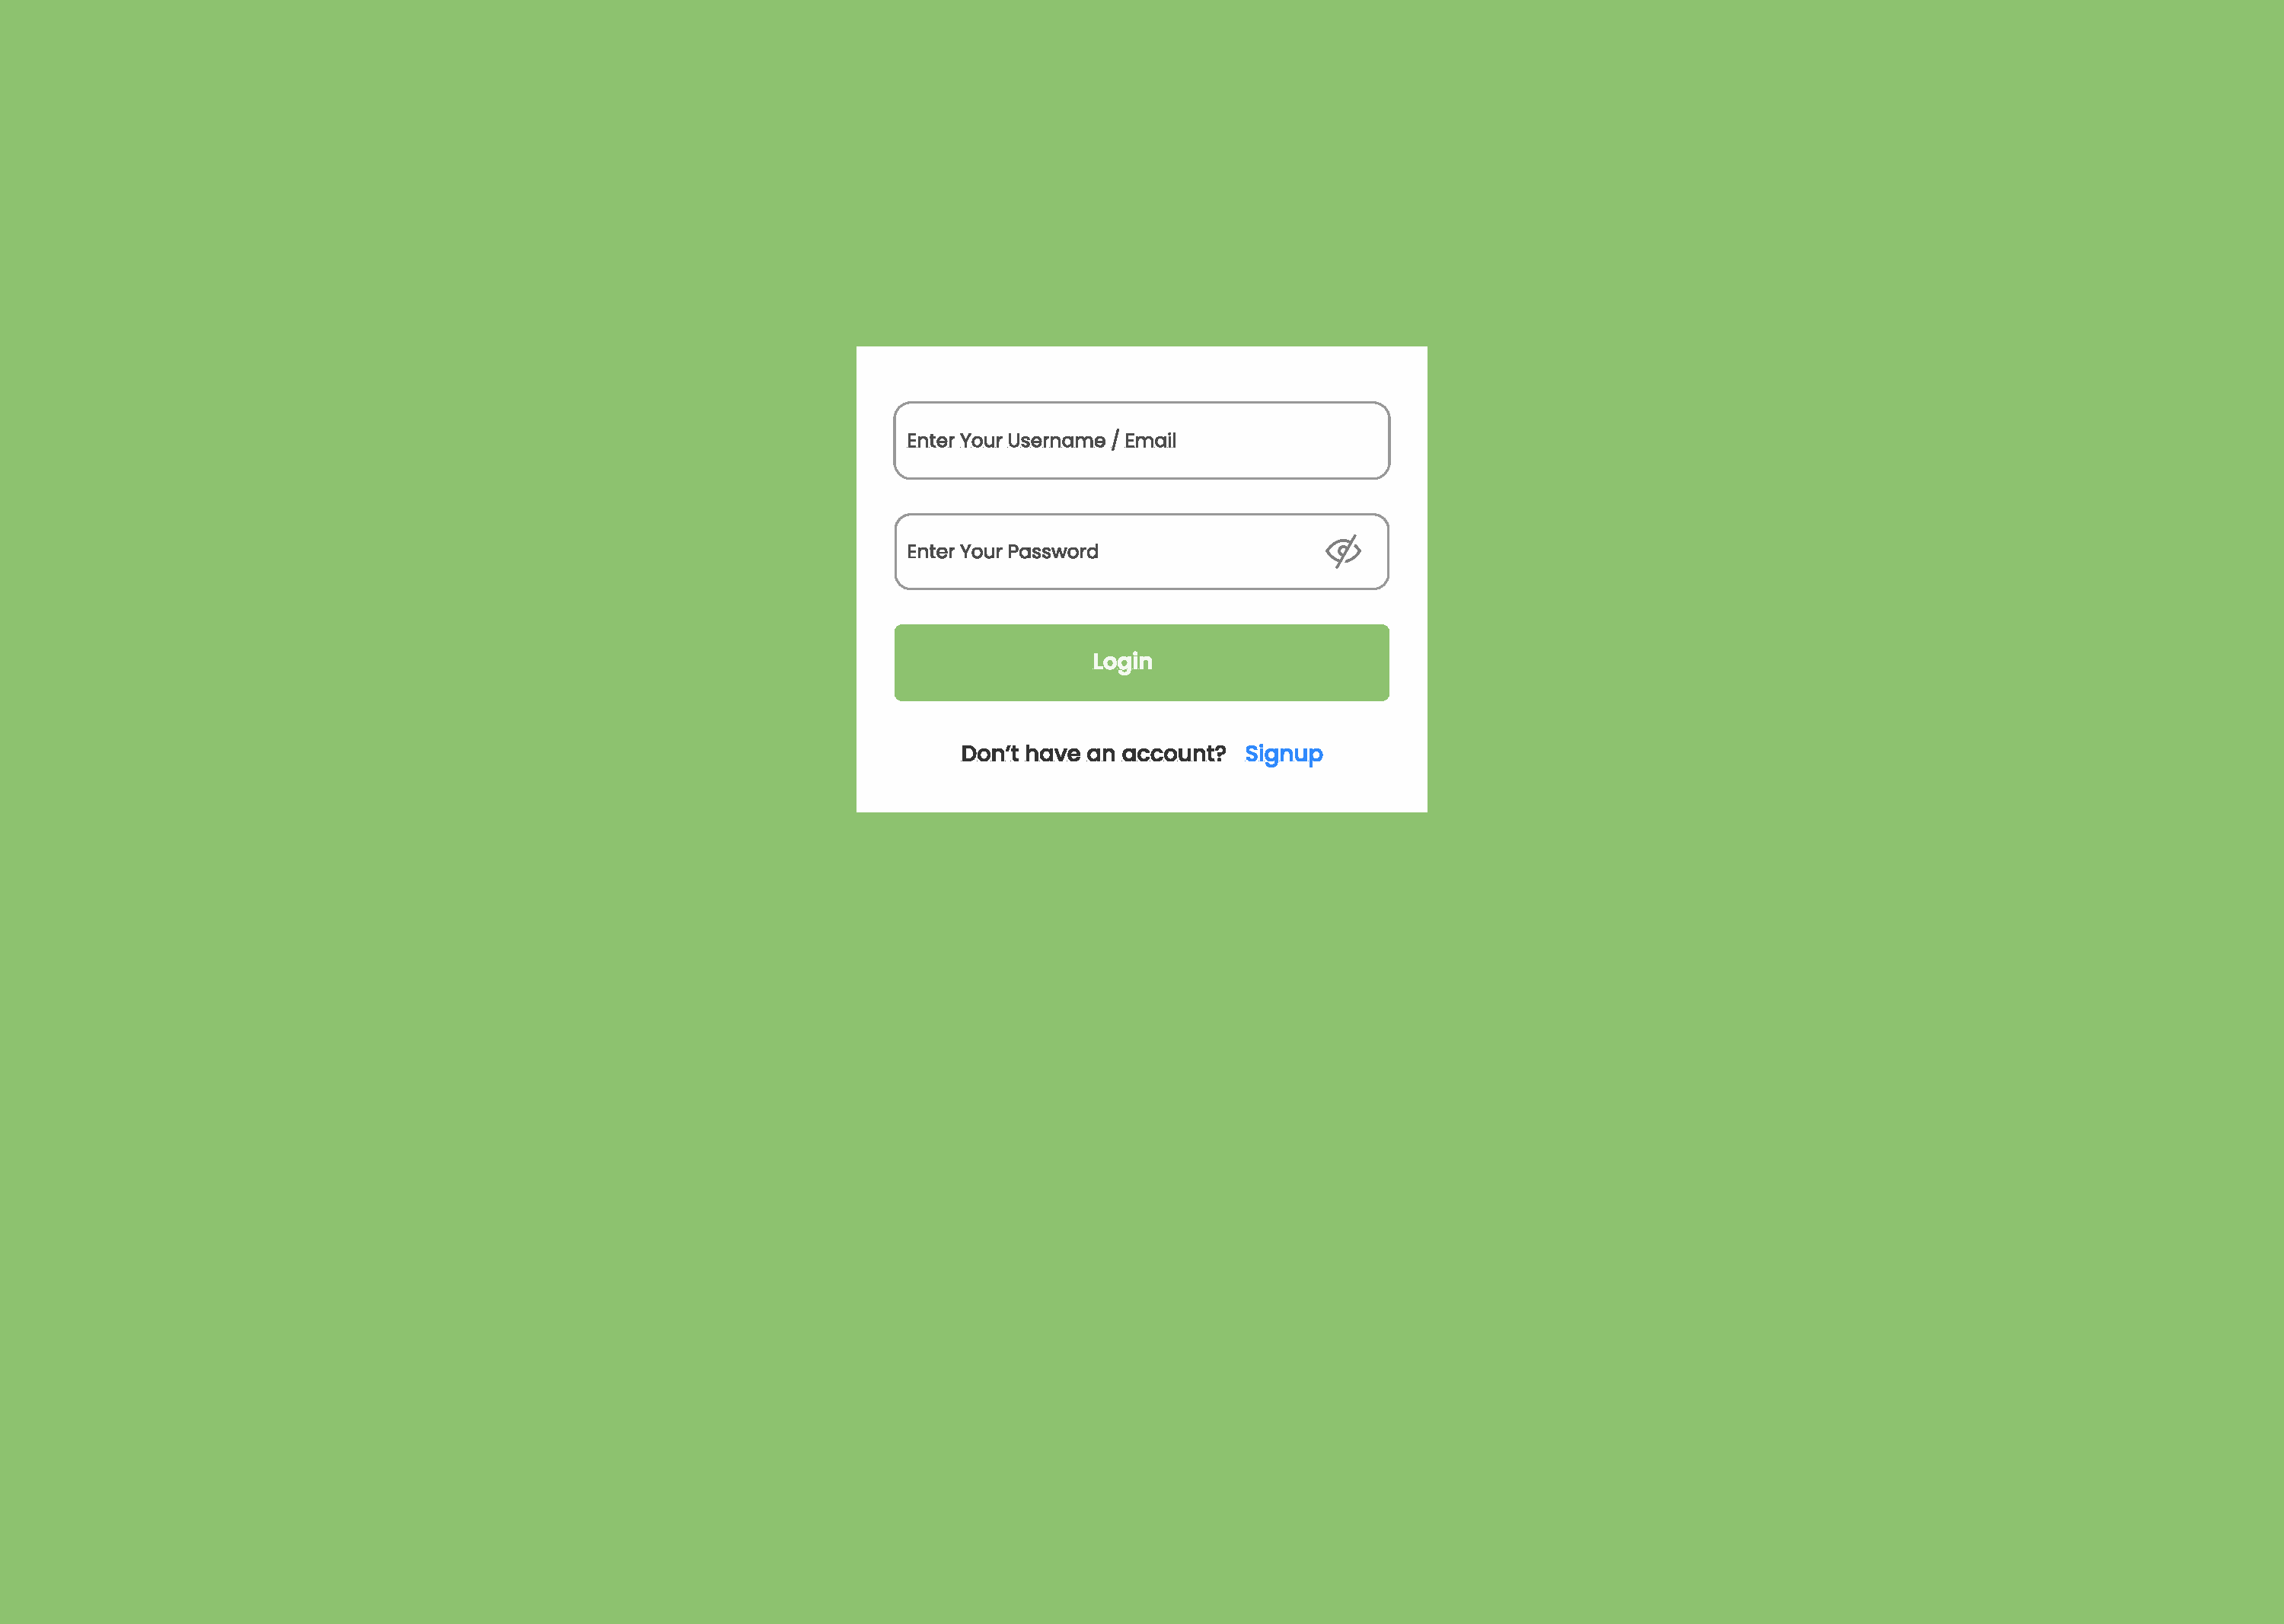
\includegraphics[width=.95\linewidth]{diagrams/1.login-old.pdf}
    \caption{Login Page}
    \label{fig:sub1}
  \end{subfigure}%
  \begin{subfigure}{.5\textwidth}
    \centering
    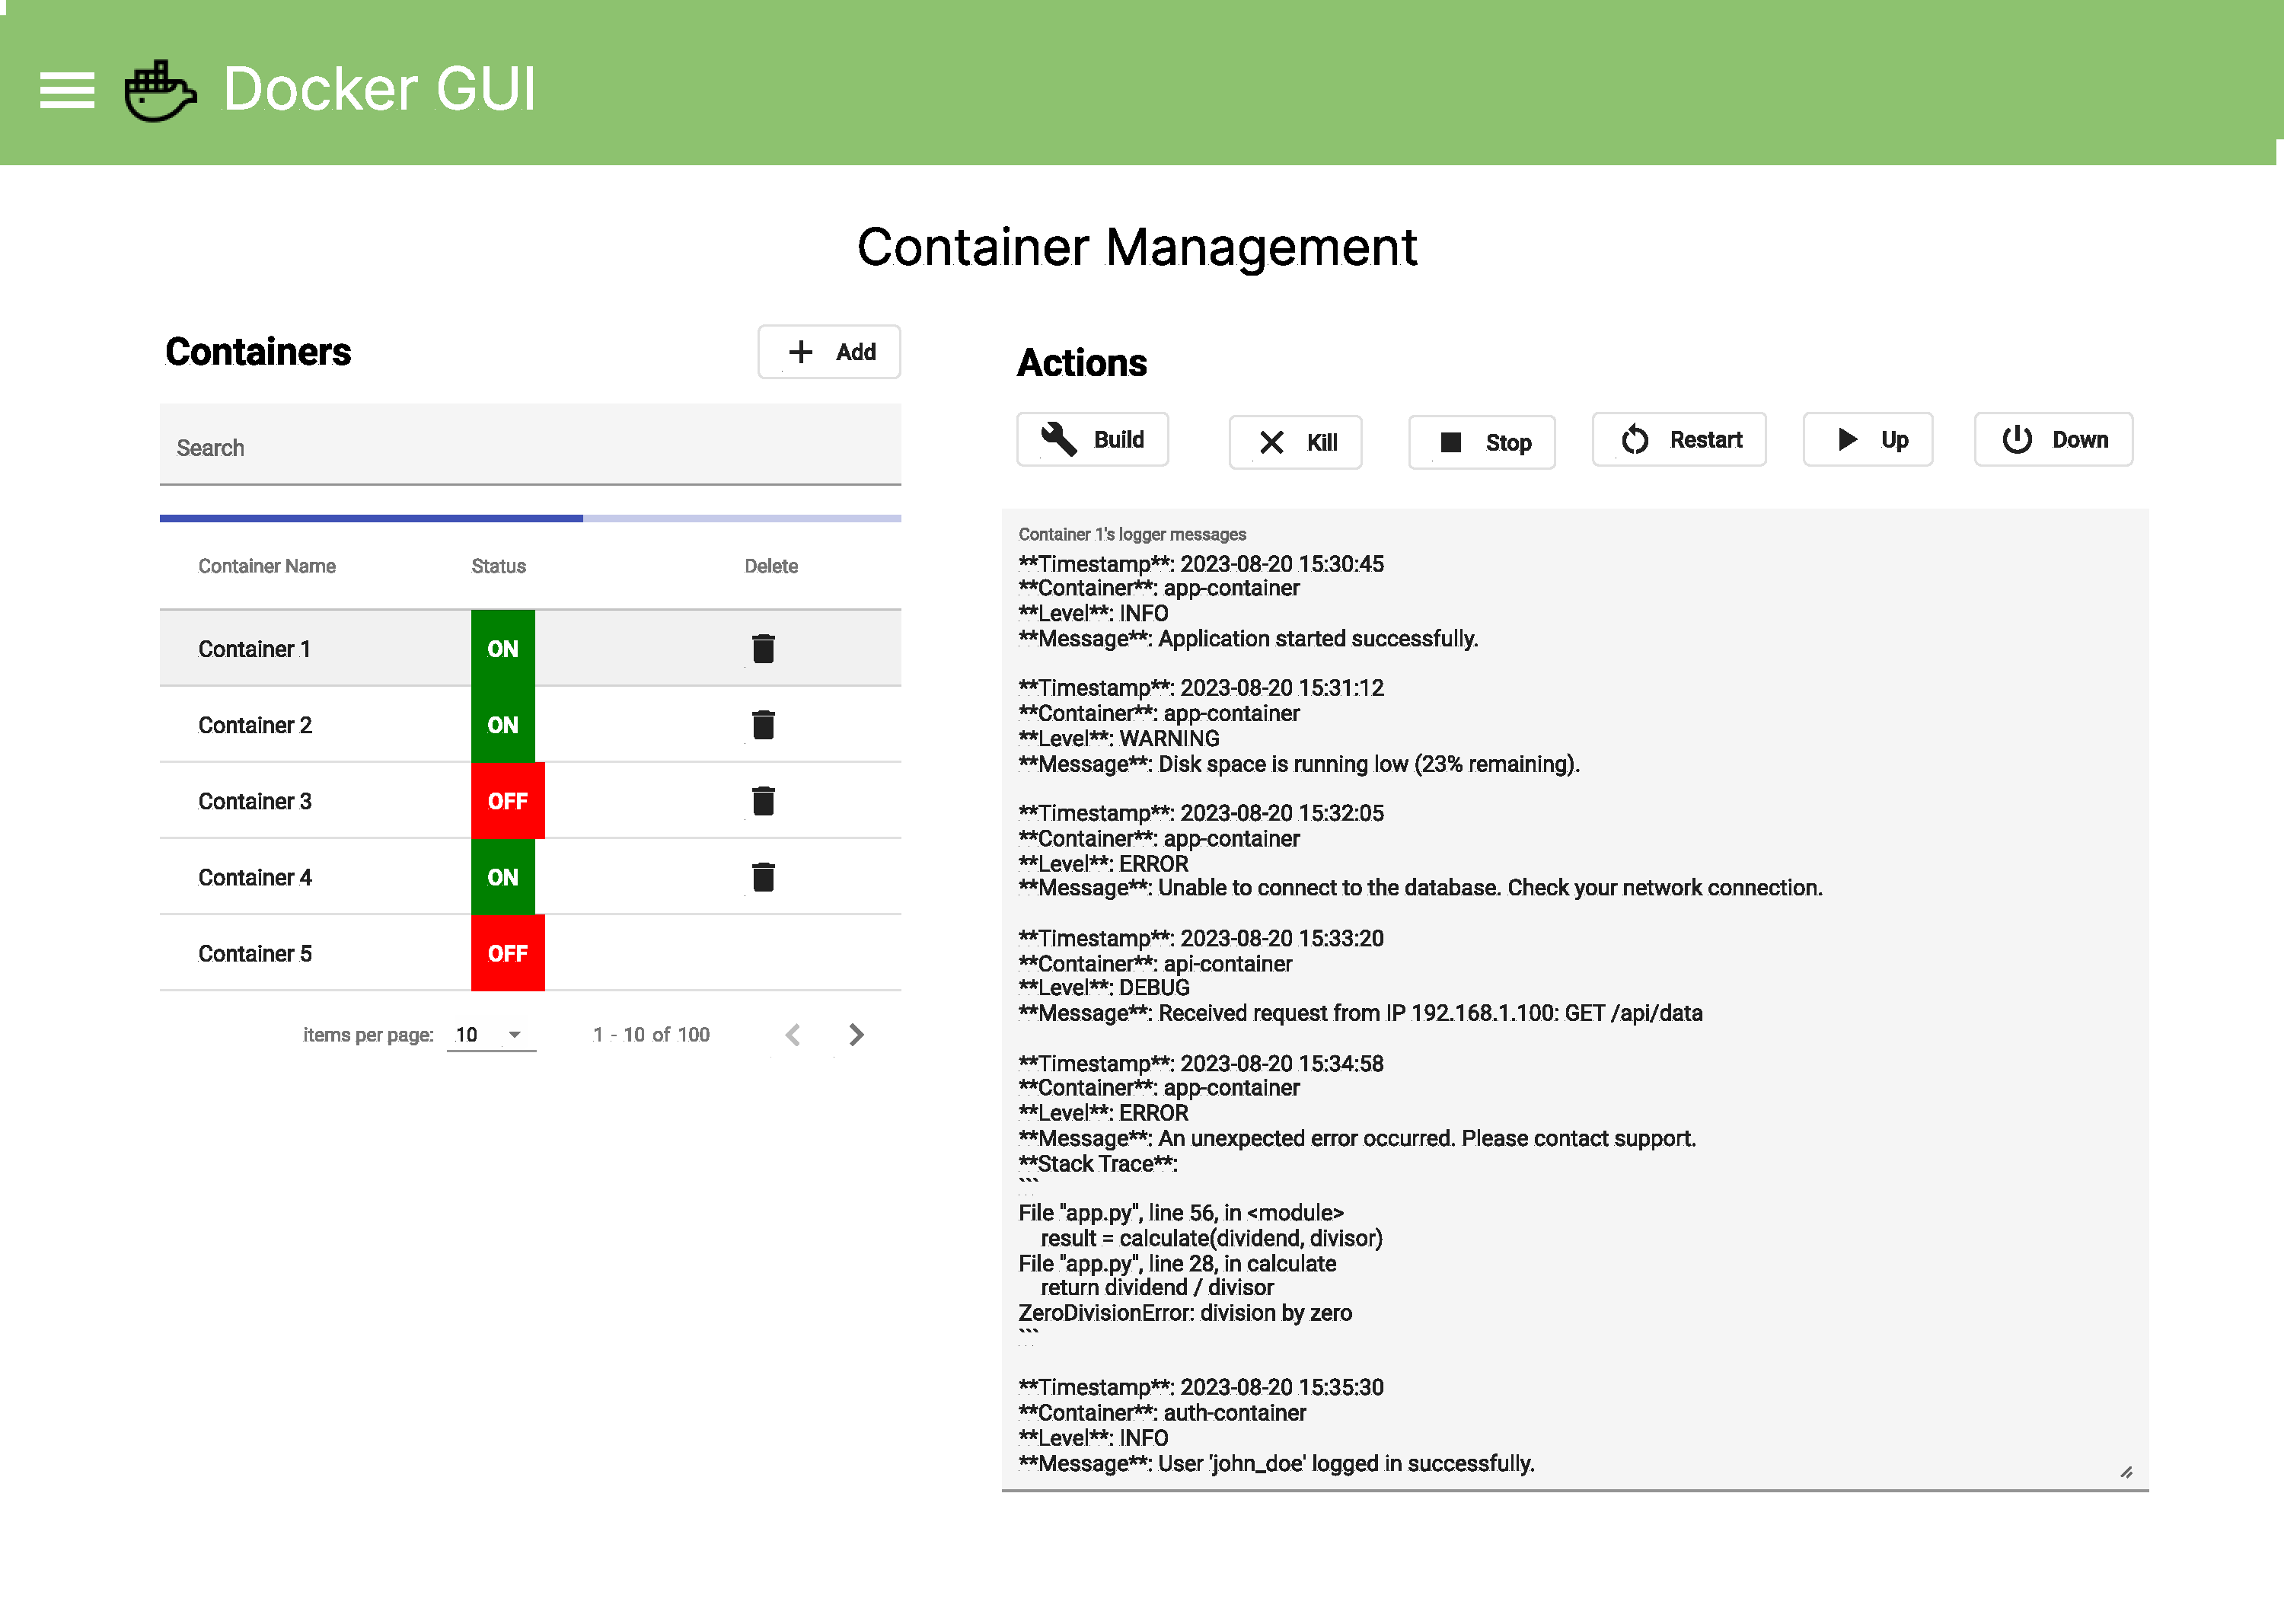
\includegraphics[width=.95\linewidth]{diagrams/3.container-old.pdf}
    \caption{Container Management Page}
    \label{fig:sub2}
  \end{subfigure}
  \caption{Non final versions, revised via Figma}
  \label{fig:login-registration-old}
\end{figure}



\subsection{Questionnaires: UEQ}
I utilized an User Experience Questionnaire (UEQ) \footnote{The link of the UEQ
is available \href{https://easy-feedback.com/docker-ui/1721729/sV3Xny}{here}.}
which assessed and measured users' enjoyment of using the application. In the
next section, I'll describe these results which can be summarized in two
diagrams.

\subsubsection{Results}
\begin{figure}[h!]
  \centering
  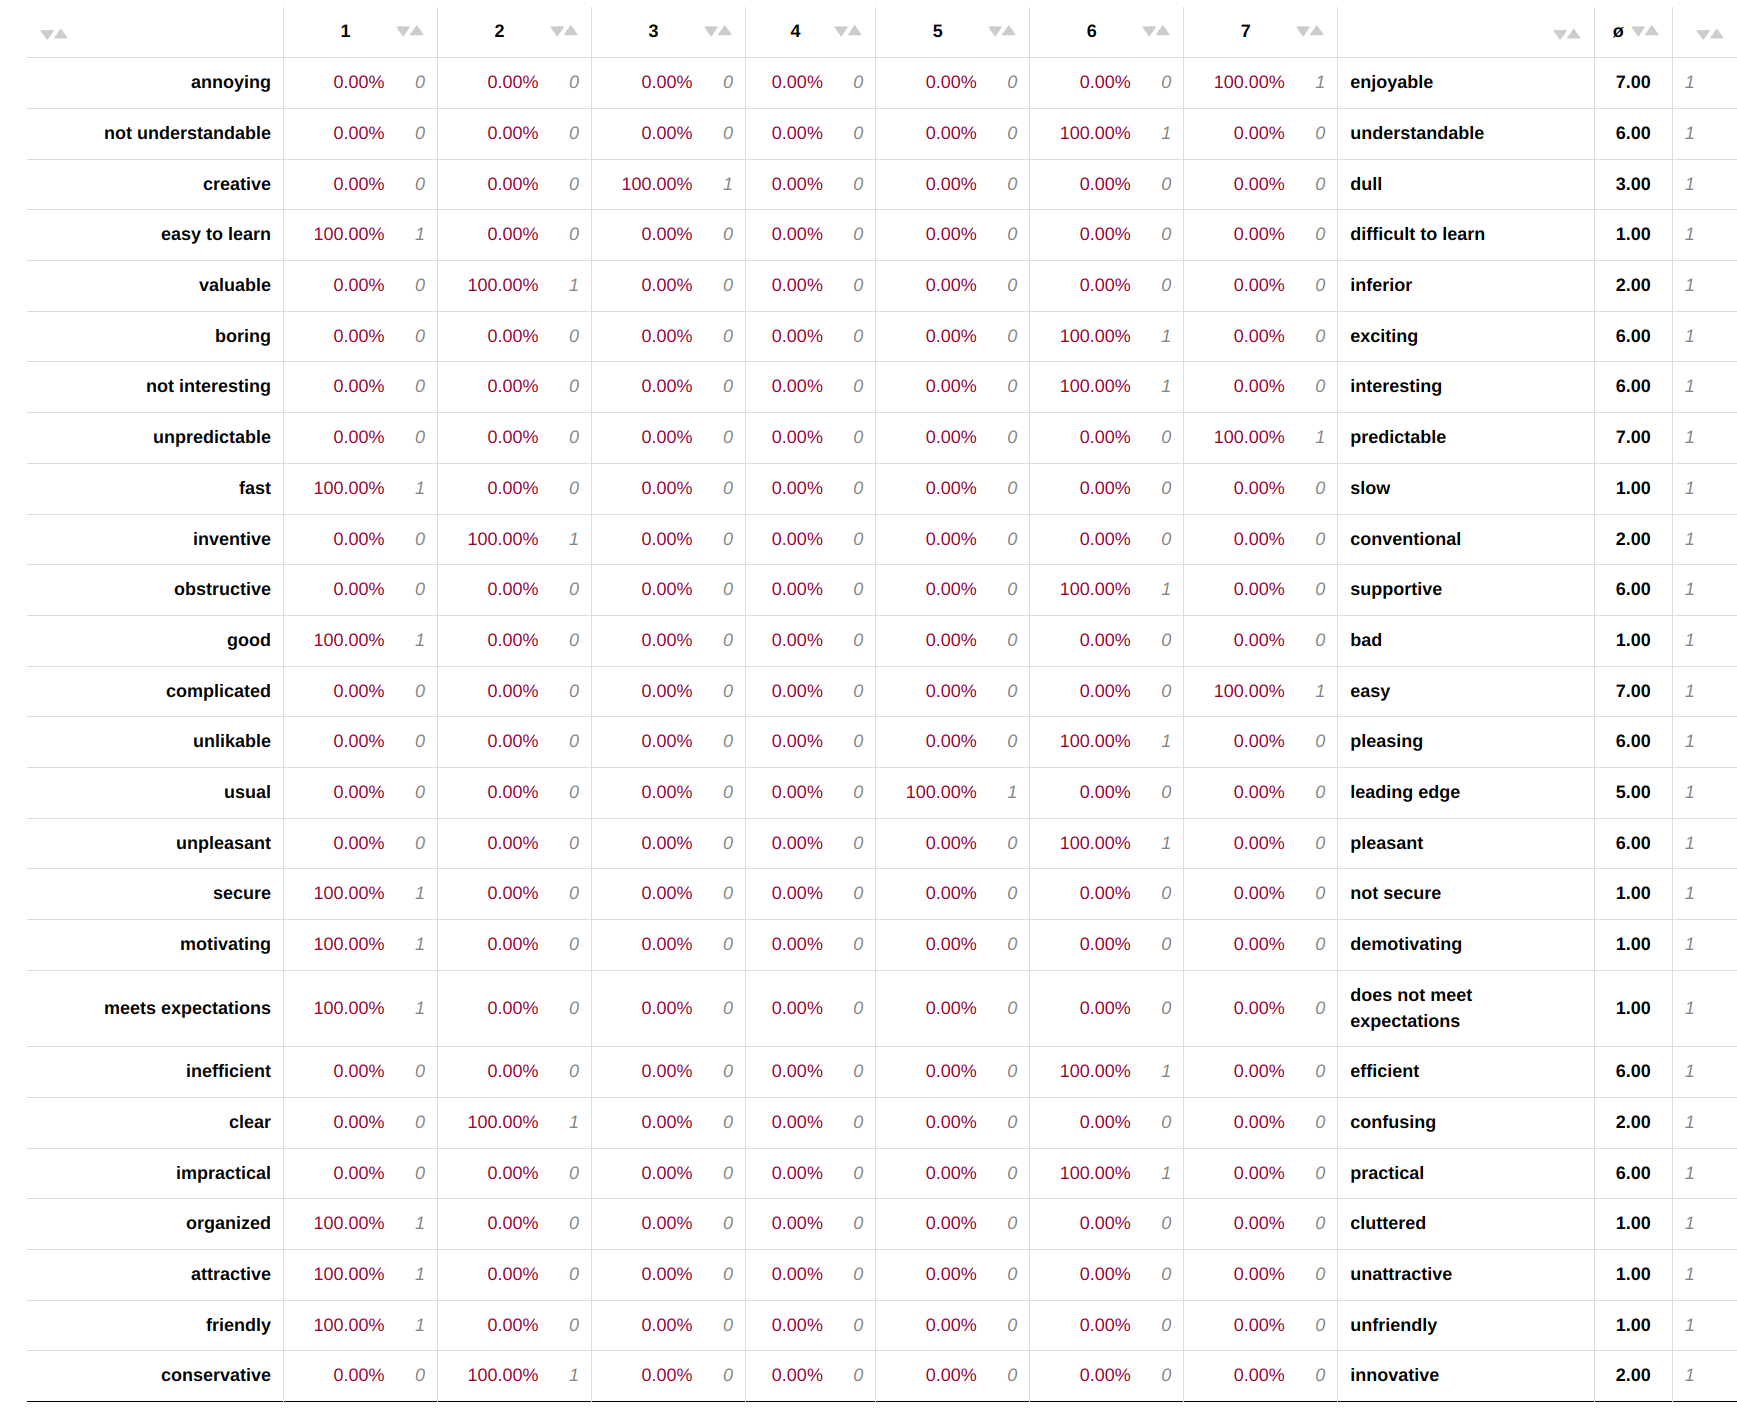
\includegraphics[scale=0.27]{survey-1}
  \caption{UEQ: Visual Representation results}
  \label{fig:ueq1}
\end{figure}

\begin{figure}[h!]
  \centering
  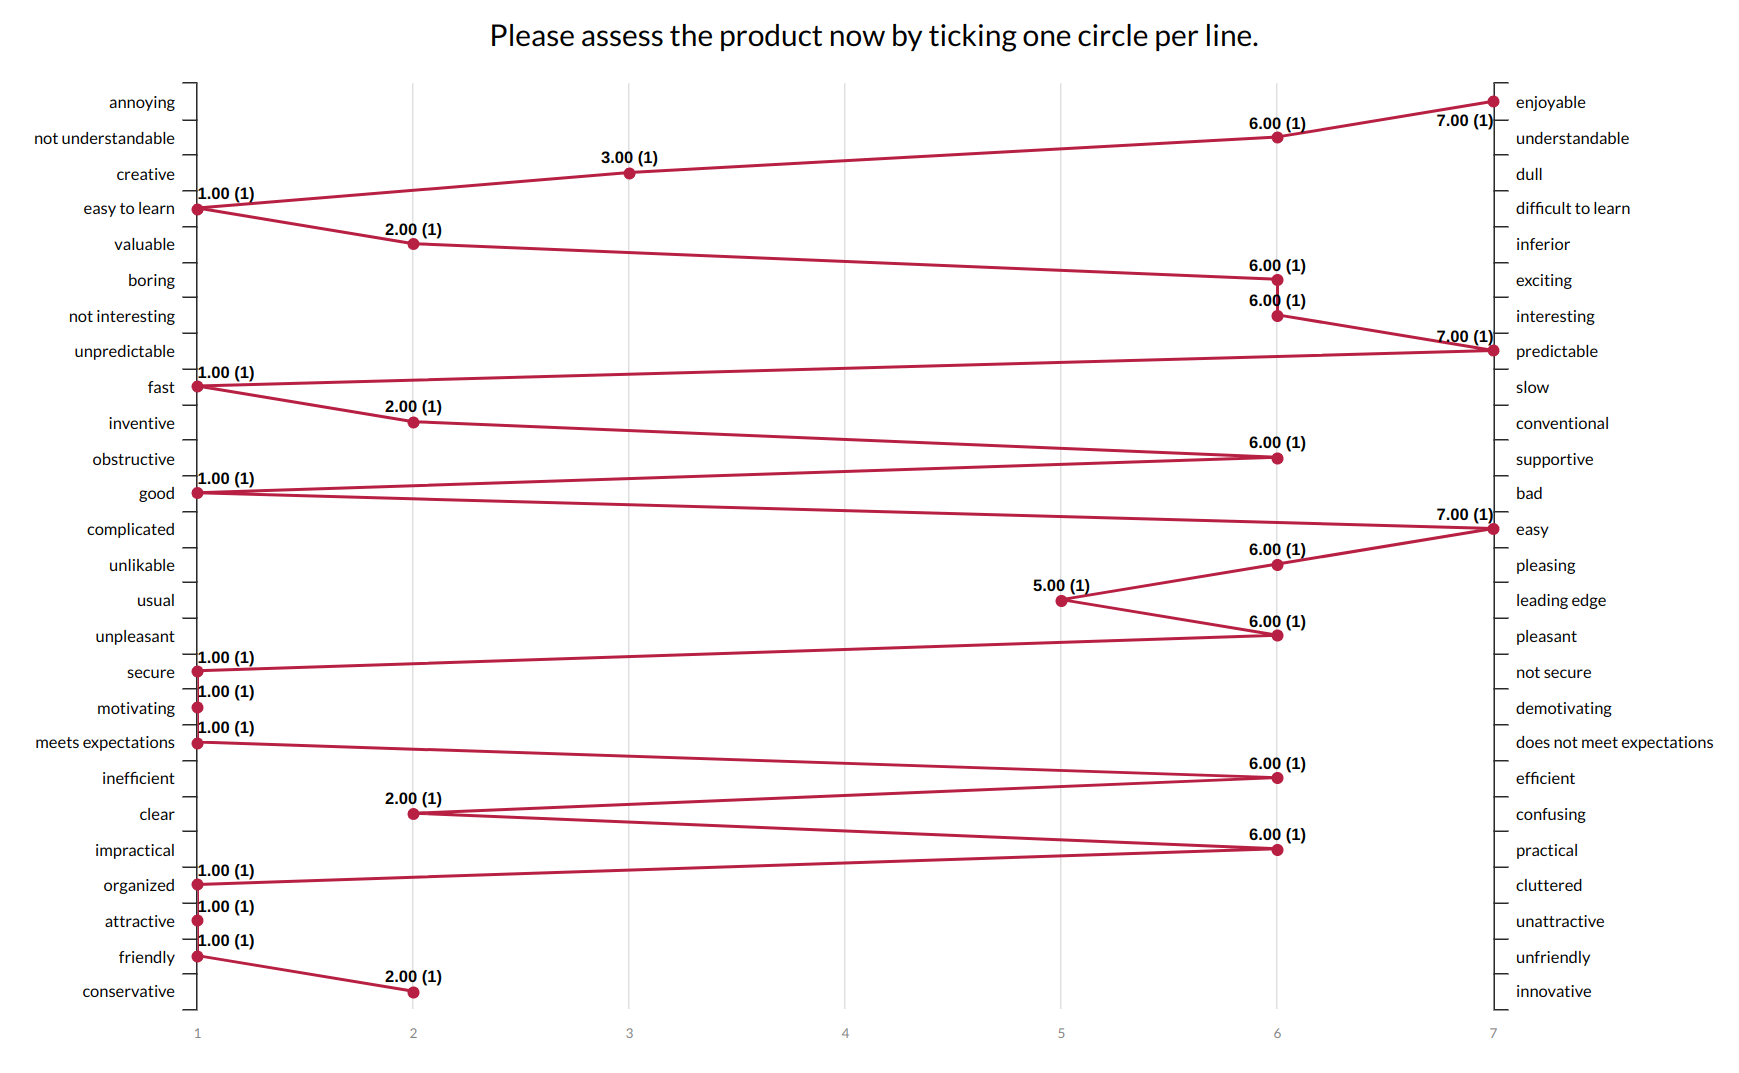
\includegraphics[scale=0.27]{survey-2}
  \caption{UEQ: Average of the results}
  \label{fig:ueq2}
\end{figure}

On the right-hand-side of Figure \ref{fig:ueq1}, it is shown the number of
people that took part in the survey and across each line there is the choice
each person made against each particular evaluated characteristic.


There were two areas that were considered unclear or cluttered and as a result
changes were made, pre-modification illustrations may be seen in Figure
\ref{fig:login-registration-old}.
\begin{itemize}
  \item Login/Registration pages were considered ambiguous.
  \item Container Management page was considered cluttered.
\end{itemize}

The second diagram, shown in Figure \ref{fig:ueq2}, shows the average of each
evaluation metric, that is the sum across all surveys for a specific 
characteristic divided by the number of total completed questionnaires. These
questions were arranged in the same order as shown in the official
documentation \footnote{UEQ homepage: https://www.ueq-online.org/.}.


\section{Deployment}
\subsection{Docker Architecture}
Diagram \ref{fig:architecture} shows the high level architectural view of the
application. This can be described as follows:
\begin{itemize}
\item \textbf{Frontend}: a variable number of clients connect using the browser
  to the Angular Frontend application, which exists in its own self contained
  Docker container.
  \begin{itemize}
  \item interaction with the UI leads to requests being made to the ExpressJS
    back-end.
  \item There exists an intermediary layer which manages data in real-time using
    SocketIO. This is used for updating the user interface dynamically as
    messages are generated by the containers.
  \item the frontend has access to local storage using the Web Cache which
    allows the user to remain logged in across browser refreshes.
  \end{itemize}
\item \textbf{Back-end}: using its own container. It speaks with the Mongo
  database via Mongoose. It also generates messages which are sent to the client
  via SocketIO.
\item \textbf{MongoDB}: deployed separately as its own container. It is
  primarily used for storing registration and user information which is used
  when an user logs in.
\end{itemize}

\begin{figure}[h!]
  \centering 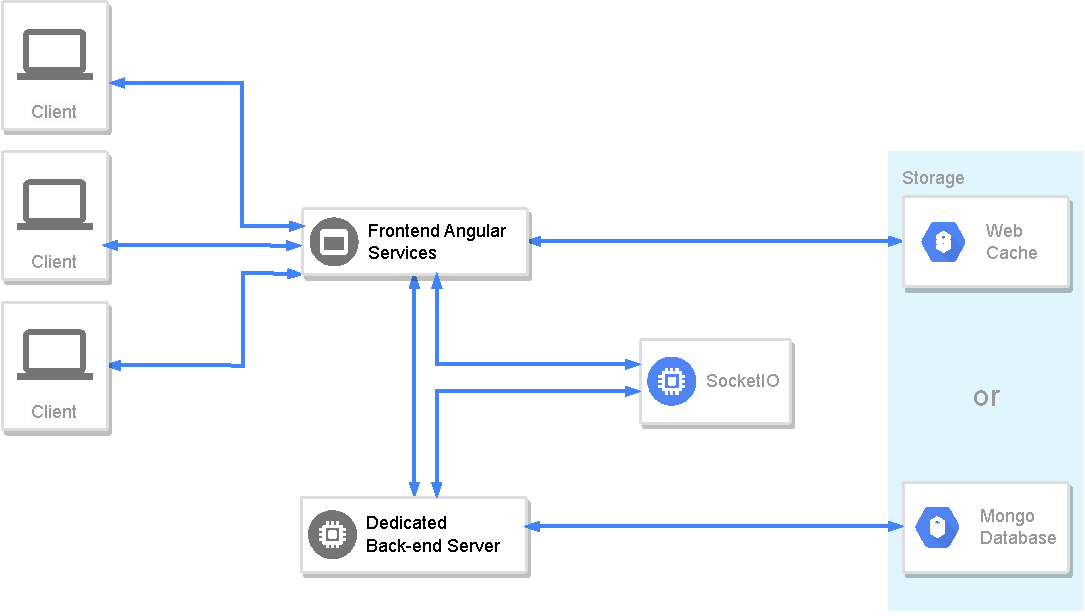
\includegraphics[scale=0.70]{diagrams/architecture.drawio.pdf}
  \caption{Docker Architecture}
  \label{fig:architecture}
\end{figure}

\subsection{Docker deployment}
The two Docker images ({\em{docker-ui-client}} and {\em{docker-ui-server}}), are
created and uploaded to the Docker Hub \footnote{Uploaded to
https://hub.docker.com/r/razvanfv/docker-ui}.

Below is a review of how these images are generated:

\begin{lstlisting}[language=docker-compose-2,caption={Deployment to Docker Hub},breaklines=true,label={code:compose}]
version: "3.8"

# Define the services
services:
  server:
    image: razvanfv/docker-ui:server # based on upstream image
    container_name: docker-ui-server
    hostname: docker_compose
    working_dir: /opt/docker-projects/ # where sample projects are located
    ports:
      - "3000:3000" # port listening to
    volumes:
      - ./server-side/docker-projects:/opt/docker-projects
      - /var/run/docker.sock:/var/run/docker.sock
    environment:
      - SECRET=Thisismysecret
      - NODE_ENV=development
      - MONGO_DB_USERNAME=admin-user
      - MONGO_DB_PASSWORD=admin-password
      - MONGO_DB_HOST=database
      - MONGO_DB_PORT=
      - MONGO_DB_PARAMETERS=?authSource=admin
      - MONGO_DB_DATABASE=docker-ui
      - USING_DOCKER=true
    links:
      - database

  database: # name of the third service
    image: mongo # specify image to build container from
    container_name: docker-ui-mongo
    environment:
      - MONGO_INITDB_ROOT_USERNAME=admin-user
      - MONGO_INITDB_ROOT_PASSWORD=admin-password
      - MONGO_DB_USERNAME=admin-user1
      - MONGO_DB_PASSWORD=admin-password1
      - MONGO_DB=docker-ui
    volumes:
      - ./mongo:/home/mongodb
      - ./mongo/init-db.d/:/docker-ui-entrypoint-init-db.d/
      - ./mongo/db:/data/db
    ports:
      - "27017:27017" # specify port forewarding


  client: # name of the first service
    image: razvanfv/docker-ui:client
    container_name: docker-ui-client
    volumes:
      - /var/run/docker.sock:/var/run/docker.sock
    ports:
      - "4200:4200" # <host>:<container>
    links:
      - server

\end{lstlisting}

Listing \ref{code:compose} is a {\em{docker-compose.yml}} file which creates and
deploys three services: the \textbf{server}, the \textbf{database} and the
\textbf{client}. Below is a description of the file:
\begin{itemize}
\item \textbf{image}: the context used as an image. Can be remote, on Docker Hub
  or local to a {\em{Dockerfile}}.
\item \textbf{working\_dir}: sets the working directory of the container that is
  created.
\item \textbf{environment}: variables needed to configure the service. Could be
  for instance configuration parameters needed by MongoDB to create the
  database.
\item \textbf{volumes}: are a mechanism for persisting data generated by and
  used by Docker containers. It should be noted that the following line allows
  Docker inside the container to communicate with the host.
  $$/var/run/docker.sock:/var/run/docker.sock$$
\item \textbf{ports}: links ports between the host and the container in such a
  way to allow inter-communication.
\item \textbf{links}: There exists a dependency between the server and the
  database, as well as one between the client and the server which is defined
  via the {\textbf{links}} keyword. This make the corresponding services
  reachable across the network.
\end{itemize}

\section{Conclusion}
To conclude, it follows a list of learning outcomes that were attained as a
result of having completed this project.

\paragraph{Containerization.}
The concepts related to \textbf{containerization} were particularly interesting.
I learnt about how to package an application into smaller images each deployed
independently through the use of containers. As an example, I was able to obtain
familiarity with the mechanisms used by Docker to deploy a somewhat non trivial
application around a variable number of services.

\paragraph{Docker.}
As it was already mentioned, I hosted and deployed the application to Docker
Hub. As a consequence, I learnt more thorough knowledge of images as the prime
building block, created directly through the use of {\em{Dockerfile}}s. These
images were instantiated to create containers. These containers communicate with
one another and run the application. Having implemented functionality leveraging
these concepts through the use of docker-compose files was particularly
exciting.

\paragraph{Docker Compose.}
The project examples which were provided enabled the user to perform common
operations on the corresponding containers. These operations leveraged the use
of a Javascript library known as {\em{docker-compose}}. The implemented
functionality involved tasks such as building, running or removing a container.

\paragraph{Future work.}
Keeping in mind the importance and inter-dependence of services with the
docker-compose files, perhaps further work might involve highlighting better the
status of each service. This would support the user to understand more
thoroughly and easily the status of each executed docker-compose file.
Currently, a project is considered {\em{up}} when all the services which compose
it have been started successfully. In some cases this is inconvenient as it
requires the user to carefully check the project's logging information in order
to fully individuate the issue.

\paragraph{Angular.}
On the other side, having worked with Angular allowed me to learn relatively
more advanced concepts. For example, I made use of guards to protect pages and
redirect to the login page in case the user would not be signed in. Furthermore,
the JsonWebToken was used to keep the user authenticated across page navigation.
To be more precise, during refreshes of the website, user authentication
information would normally get lost but by using these tokens the information is
securely stored and restored whenever needed.

\paragraph{Conclusion.}
As a whole, the project was particularly interesting and having developed more
thorough knowledge of both Docker and Angular, I am excited to see when these
skills will be of use in the future.


\bibliographystyle{plain}
\newpage
\printbibliography
\end{document}

